In this chapter we provide a Gray code for listing all ladders with $k$ bars. 
We define $L_{n,k}$ as the set of all canonical ladder lotteries with $n$ lines and exactly $k$ bars, where $0 \leq k \leq {n \choose 2}$. To list $L_{n,k}$, 
we define a mapping from associated diagonals to 
an inversion vector corresponding to $\pi$. We apply this mapping to a generate a Gray code for listing $L_{n,k}$. 
We then provide an algorithm for listing $L_{n}$ ordered by the number of bars from $0 \leq k \leq {n \choose 2}$ in Gray code order. 
We list $L_{n}$ by $k$ bars as follows - Let $k$ be the current number of bars in the ladder; $k$ is initialized to $0$ and terminates at ${n \choose 2}$. 
We first list $L_{n,k}$ before we list the first ladder in $L_{n, k+1}$. When listing ladders by $k$ 
bars, we define minimal change as the relocation 
of a bar; relocating a bar is equivalent to removing one bar and adding another bar.  



\section{Listing all ladders with $n$ lines and $k$ bars in Gray code order}
 In Chapter 2, we discussed Effler-Ruskey's algorithm and Walsh's Gray code for listing $S_{n,k}$. 
In this section, we focus on Walsh's Gray code for listing $L_{n,k}$ by applying a minimal amount of change between subsequent ladders. We 
relocate a bar to transition from one ladder in $L_{n,k}$ to the next ladder in $L_{n,k}$. Recall, relocating a bar is the same as 
adding one bar and removing another bar.\par  
An $n$ part composition of a non negative integer $k$, is an $n$ tuple $g=(g_{1}, g_{2}, \dots g_{n})$ whose sum adds to $k$. We 
say $g$ is the \emph{bar vector of $CL(\pi_{n+1})$} when we map $g$ to a canonical ladder as follows - For each 
index $x$ in $g$, $x$ is mapped to the associated diagonal of $((n+1)-x) + 1$. Furthermore, $g_{x}$ equals the number of bars along the associated 
diagonal of element $((n+1)-x) + 1$. To see the mapping of $g$ to the associated diagonals, refer to Figure~\ref{Fig:gToLadder}.\par 
\begin{figure}
  \centering
  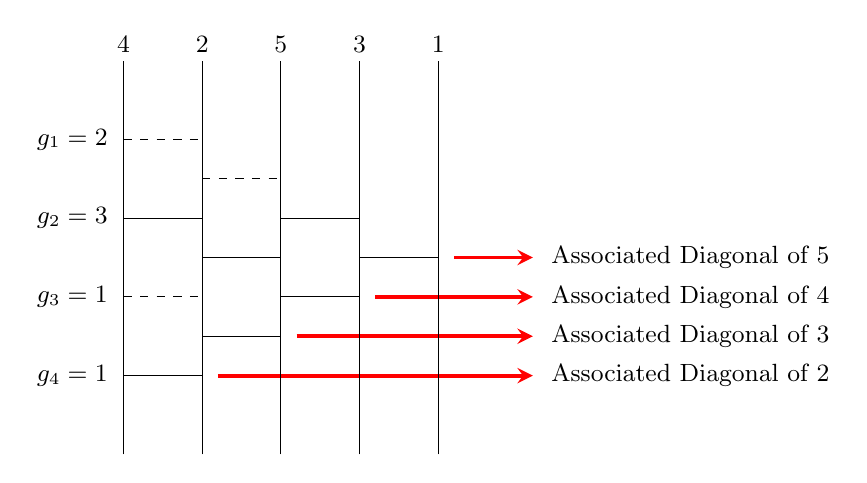
\begin{tikzpicture}
    \draw(0, 0) to (0, 5);
      \draw[dashed](0, 4) -- (1, 4);
      \draw(0, 3) to (1, 3);
      \draw[dashed](0, 2) -- (1, 2);
      \draw(0, 1) to (1, 1);
        \draw[-stealth, red, line width=.5mm](1.2, 1) -- (5.2, 1);
        \node at(7.2, 1){\small{Associated Diagonal of $2$}};
    \draw(1, 0) to (1, 5);
      \draw[dashed](1, 3.5) -- (2, 3.5);
      \draw(1, 2.5) to (2, 2.5);
      \draw(1, 1.5) to (2, 1.5);
      \draw[-stealth, red, line width=.5mm](2.2, 1.5) -- (5.2, 1.5);
        \node at(7.2, 1.5){\small{Associated Diagonal of $3$}};
    \draw(2, 0) to (2, 5);
      \draw(2, 3) to (3, 3);
      \draw(2, 2) to (3, 2);
       \draw[-stealth, red, line width=.5mm](3.2, 2) -- (5.2, 2);
        \node at(7.2, 2){\small{Associated Diagonal of $4$}};
    \draw(3, 0) to (3, 5);
      \draw(3, 2.5) to (4, 2.5);
      \draw[-stealth, red, line width=.5mm](4.2, 2.5) -- (5.2, 2.5);
      \node at(7.2, 2.5){\small{Associated Diagonal of $5$}};
    \draw(4, 0) to (4, 5);

    \node at(-0.65, 4){\small{$g_{1}=2$}};
    \node at(-0.65, 3){\small{$g_{2}=3$}};
    \node at(-0.65, 2){\small{$g_{3}=1$}};
    \node at(-0.65, 1){\small{$g_{4}=1$}};

    \node at(0, 5.2){\small{$4$}};
    \node at(1, 5.2){\small{$2$}};
    \node at(2, 5.2){\small{$5$}};
    \node at(3, 5.2){\small{$3$}};
    \node at(4, 5.2){\small{$1$}};
  \end{tikzpicture}
  \caption{Mapping of the composition $(2,3,1,1)$ to the associated diagonals of $CL(4,2,5,3,1)$}
  \label{Fig:gToLadder}
\end{figure}
$g$ is $(m_{1}, \dots, m_{n})$ bounded, if for each $g_{x}$, $0 \leq g_{x} \leq m_{x}$ where $m_{x}=(n+1)-x$; 
we let $m_{x}$ be the fixed upper bound on $g$ such that $g_{x} \leq m_{x}$. 
We let $0$ be the fixed lower bound on $g$ 
such that $0 \leq g_{x}$. We let $k-(g_{x+1}+ \dots +g_{n})$ be the fluid upper bound on $g$ such that $g_{x} \leq k-(g_{x+1}+ \dots +g_{n})$. 
We let $k-(g_{x+1}+ \dots +g_{n}) - (m_{1} + \dots + m_{x-1})$ be the fluid lower bound on $g$ such that 
$k-(g_{x+1} + \dots + g_{n}) - (m_{1} + \dots + m_{x-1}) \leq g_{x}$. We let the maximum value of $g_{x}=min(m_{x}, k-(g_{x+1}+ \dots + g_{n}))$. 
We let the minimum value of $g_{x}=max(0, k-(g_{x+1} + \dots +g_{n})-(m_{1} + \dots + m_{x-1}))$. For example, suppose $k=9$, $n=5$, $x=3$, $g=$(\underline{  },\underline{  },\underline{  },$1$)
 and $m=(4,3,2,1)$. The minimum value of $g_{3}=max(0, 9 - 1 - (4+3))$ and the maximum value of $g_{3}=min(2, 9-1)$. 
 Walsh's Gray Code for listing compositions is as follows follows - We start with the lexicographically largest composition $(k,0, \dots ,0)$. We define the 
 \emph{last value of $g_{x}$} as either the max or min value of $g_{x}$ 
 depending on whether the suffix $(g_{x+1}+ \dots +g_{n})$ is odd or even. If the suffix is of odd parity, then the last value of $g_{x}$ is 
 equal to the $max(0, k-(g_{x+1} + \dots + g_{n})-(m_{1} + \dots + m_{x-1}))$. If the suffix is of even parity, then the last value of 
 $g_{x}$ is equal to the $min(m_{x}, k-(g_{x+1} + \dots + g_{n}))$. We 
 scan left to right, starting at $x=2$, to find the first $g_{x}$ that is not at its last value; if no such $g_{x}$ exists, then the current composition 
 is the last one. Once found, $g_{x}$ is increased by $1$ if $(g_{x+1} + \dots + g_{n})$ is even, else $g_{x}$ is decreased by $1$. Because we are 
 obligated to ensure $g$ sums to $k$, when $g_{x}$ is incremented or decremented by $1$, then we must decrement or increment some $(g_{1}, \dots g_{w} \dots, g_{x-1})$ 
 by $1$. We determine which $g_{w}$ to change by scanning right to left, starting at $g_{x-1}$ until we find the smallest $w<x$ such that 
 $g_{w}$ can be incremented by $1$ if $g_{x}$ was decremented by $1$, or decremented by $1$ if $g_{x}$ was incremented by $1$.\par 
 Although we use the same sequencing rule as Walsh to list the compositions, our mapping of the composition 
 to the associated diagonals lends to a different ordering $S_{n+1,k}$ than that of Walsh's ordering of $S_{n+1,k}$. Note, 
 that Walsh's $g$ composition is the same as our bar vector, however we map our bar vector to the associate diagonals of the 
 canonical ladder. 
 In Table~\ref{Table:diffPermsSameComp} we see the composition listing for $n=4$ and $k=2$, 
 Walsh's listing of $S_{5,2}$, and our listing of permutations of $S_{5,2}$, derived from our mapping of the bar vector to the canonical ladder. 
 \begin{table}[h]
  \centering
  \begin{tabular}{|p{4cm}|p{4cm}|p{4cm}|}
    
    \hline 
    $g$/Bar vector & Walsh's Permutation & Our Permutation \\ 
    \hline 
    \hline 
    $(2,0,0,0)$ & $(3,1,2,4,5)$ & $(1,2,5,3,4)$ \\ 
    \hline 
    $(1,1,0,0)$ & $(2,3,1,4,5)$ & $(1,2,4,5,3)$ \\ 
    \hline 
    $(0,2,0,0)$ & $(1,4,2,3,5)$ & $(1,4,2,3,5)$ \\ 
    \hline 
    $(0,1,1,0)$ & $(1,3,4,2,5)$ & $(1,3,4,2,5)$ \\ 
    \hline 
    $(1,0,1,0)$ & $(2,1,4,3,5)$ & $(1,3,2,5,4)$ \\ 
    \hline 
    $(0,0,2,0)$ & $(1,2,5,3,4)$ & $(3,1,2,4,5)$\\ 
    \hline 
    $(0,0,1,1)$ & $(1,2,4,5,3)$ & $(2,3,1,4,5)$ \\ 
    \hline 
    $(0,1,0,1)$ & $(1,4,3,5,2)$ & $(2,1,4,3,5)$ \\ 
    \hline 
    $(1,0,0,1)$ & $(2,1,3,5,4)$ & $(2,1,3,5,4)$ \\ 
    \hline 

  \end{tabular}
  \caption{Table comparing the listing of permutations with the same composition}
  \label{Table:diffPermsSameComp}
 \end{table}
We have claimed we can list compositions $g$ in such a way that we can list $L_{n+1,k}$ by mapping each $g_{x}$ to the number of bars along the associated diagonal 
of $((n+1)-x)+1$. We have yet to demonstrate the details of this mapping. If $k>0$, we define \emph{the lexicographically largest ladder} as the 
ladder such that the associated diagonal of any element $y>w$, the number of bars in $y's$ diagonal is the $min(m_{(n+1-y)+1}, k-\text{the number of bars along the associated diagonals of } n+1,n,\dots,y+1)$.
 We start with the lexicographically largest ladder and the corresponding lexicographically largest $g$. To list $g$, we use the same 
 sequencing rule as Walsh. To list $L_{n+1, k}$, we let $x'=(n+1)-x+1$ and we let $w'=(n+1)-w+1$, where $x \neq w$. We add or remove one bar from the associated diagonal of $x'$ and remove or add another bar 
 from the associated diagonal of $w'$; we always do the inverse operation on $x'$ and $w'$ in order to 
 ensure $k$ does not change. When we remove a bar, we do so from the top left of an associated 
 diagonal, and when we add a bar, we do so to the bottom right of an associated diagonal. 
 To find our $x'$ value, we scan $g$ from $(g_{2}, \dots, g_{n})$ until we find a $g_{x}$ that is not at its last value. We then 
 increment $g_{x}$ by $1$ and add a bar to the associated diagonal of $x'$ if the suffix $(g_{x+1} + \dots + g_{n})$ is even. Otherwise 
 we decrement $g_{x}$ by $1$ and remove a bar from the associated diagonal of $x'$. Once we have added or removed a bar from $x'$ we scan the 
 prefix $(g_{x-1}, \dots, g_{1})$ from 
 right to left, to find the smallest $w$ value less than $x$ such that $g_{w}$ is not at its last value. If $g_{x}$ was incremented 
 by $1$, then $g_{w}$ is decremented by $1$ and a bar along the associated diagonal of $w'$ is removed. If $g_{x}$ was 
 decremented by $1$, then $g_{w}$ is incremented by $1$ and a bar along the associated diagonal of $w'$ is added. 
 We use Equation~\ref{GetCoordinates3} to calculate the row and column of the bar to be added or removed. 

 \begin{equation}\label{GetCoordinates3}
  \resizebox{.9\textwidth}{!}{
    (row,column)=
    \begin{cases}
      ((n+x)-g(x), (n+1-x)-g(x)+1) & \text{if a bar is being removed} \\
      ((n+x-1)-g(x), (n+1-x)-g(x)) & \text{if a bar is being added}
    \end{cases}
  }
 \end{equation} 

 In Figure~\ref{Fig:LnK} we provide the listing of $L_{5,2}$ using Walsh's Gray code for listing $g$ and our mapping of $g$ to the associated diagonals of 
 the canonical ladder.\pagebreak 
 \begin{figure}[ht]
  \centering
  \begin{minipage}{.3\textwidth}
    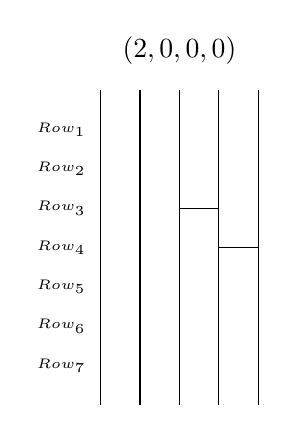
\begin{tikzpicture}
      \node at (1, 4.5){$(2,0,0,0)$};
      \draw(0, 0) to (0, 4);
      \draw(0.5, 0) to (.5, 4);
      \draw(1, 0) to (1, 4);
        \draw(1, 2.5) to (1.5, 2.5);
      \draw(1.5, 0) to (1.5, 4);
        \draw(1.5, 2) to (2, 2);
      \draw(2, 0) to (2, 4);
      \node at(-0.5, 3.5){\tiny{$Row_{1}$}};
      \node at(-0.5, 3.0){\tiny{$Row_{2}$}};
      \node at(-0.5, 2.5){\tiny{$Row_{3}$}};
      \node at(-0.5, 2.0){\tiny{$Row_{4}$}};
      \node at(-0.5, 1.5){\tiny{$Row_{5}$}};
      \node at(-0.5, 1.0){\tiny{$Row_{6}$}};
      \node at(-0.5, 0.5){\tiny{$Row_{7}$}};
    \end{tikzpicture}
  \end{minipage}
  \begin{minipage}{.3\textwidth}
    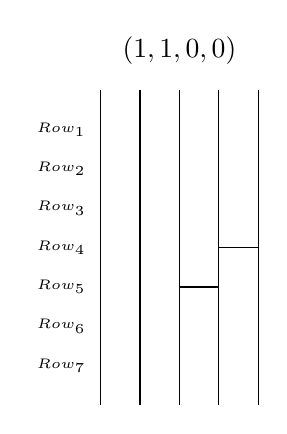
\begin{tikzpicture}
      \node at (1, 4.5){$(1,1,0,0)$};
      \draw(0, 0) to (0, 4);
      \draw(0.5, 0) to (0.5, 4);
      \draw(1, 0) to (1, 4);
        \draw(1, 1.5) to (1.5, 1.5);
      \draw(1.5, 0) to (1.5, 4);
        \draw(1.5, 2) to (2, 2);
      \draw(2, 0) to (2, 4);

     \node at(-0.5, 3.5){\tiny{$Row_{1}$}};
      \node at(-0.5, 3.0){\tiny{$Row_{2}$}};
      \node at(-0.5, 2.5){\tiny{$Row_{3}$}};
      \node at(-0.5, 2.0){\tiny{$Row_{4}$}};
      \node at(-0.5, 1.5){\tiny{$Row_{5}$}};
      \node at(-0.5, 1.0){\tiny{$Row_{6}$}};
      \node at(-0.5, 0.5){\tiny{$Row_{7}$}};
    \end{tikzpicture}
  \end{minipage}
  \begin{minipage}{.3\textwidth}
    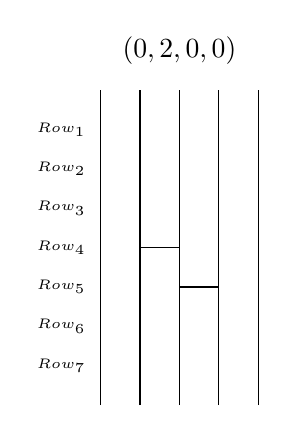
\begin{tikzpicture}
      \node at (1, 4.5){$(0,2,0,0)$};
      \draw(0, 0) to (0, 4);
      \draw(0.5, 0) to (0.5, 4);
        \draw(0.5, 2) to(1, 2);
      \draw(1, 0) to (1, 4);
        \draw(1, 1.5) to (1.5, 1.5);
      \draw(1.5, 0) to (1.5, 4);
      \draw(2, 0) to (2, 4);

     \node at(-0.5, 3.5){\tiny{$Row_{1}$}};
      \node at(-0.5, 3.0){\tiny{$Row_{2}$}};
      \node at(-0.5, 2.5){\tiny{$Row_{3}$}};
      \node at(-0.5, 2.0){\tiny{$Row_{4}$}};
      \node at(-0.5, 1.5){\tiny{$Row_{5}$}};
      \node at(-0.5, 1.0){\tiny{$Row_{6}$}};
      \node at(-0.5, 0.5){\tiny{$Row_{7}$}};
    \end{tikzpicture}
  \end{minipage}

  
  \begin{minipage}{.3\textwidth}
    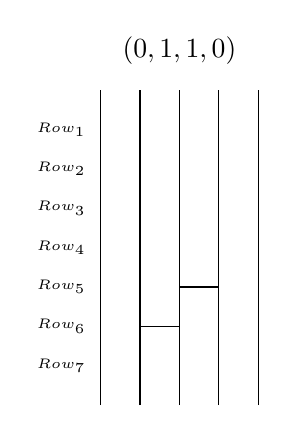
\begin{tikzpicture}
      \node at (1, 4.5){$(0,1,1,0)$};
      \draw(0, 0) to (0, 4);
      \draw(0.5, 0) to (.5, 4);
        \draw(0.5, 1) to (1, 1);
      \draw(1, 0) to (1, 4);
        \draw(1, 1.5) to (1.5, 1.5);
      \draw(1.5, 0) to (1.5, 4);
        
      \draw(2, 0) to (2, 4);
      \node at(-0.5, 3.5){\tiny{$Row_{1}$}};
      \node at(-0.5, 3.0){\tiny{$Row_{2}$}};
      \node at(-0.5, 2.5){\tiny{$Row_{3}$}};
      \node at(-0.5, 2.0){\tiny{$Row_{4}$}};
      \node at(-0.5, 1.5){\tiny{$Row_{5}$}};
      \node at(-0.5, 1.0){\tiny{$Row_{6}$}};
      \node at(-0.5, 0.5){\tiny{$Row_{7}$}};
    \end{tikzpicture}
  \end{minipage}
  \begin{minipage}{.3\textwidth}
    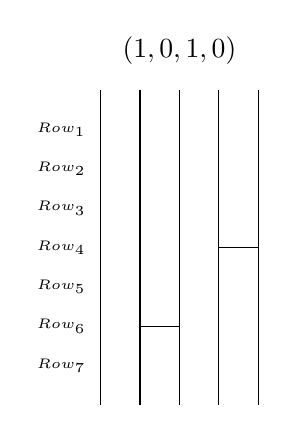
\begin{tikzpicture}
      \node at (1, 4.5){$(1,0,1,0)$};
      \draw(0, 0) to (0, 4);
      \draw(0.5, 0) to (.5, 4);
      \draw(1, 0) to (1, 4);
        \draw(0.5, 1) to (1, 1);
      \draw(1.5, 0) to (1.5, 4);
        \draw(1.5, 2) to (2, 2);
      \draw(2, 0) to (2, 4);
      \node at(-0.5, 3.5){\tiny{$Row_{1}$}};
      \node at(-0.5, 3.0){\tiny{$Row_{2}$}};
      \node at(-0.5, 2.5){\tiny{$Row_{3}$}};
      \node at(-0.5, 2.0){\tiny{$Row_{4}$}};
      \node at(-0.5, 1.5){\tiny{$Row_{5}$}};
      \node at(-0.5, 1.0){\tiny{$Row_{6}$}};
      \node at(-0.5, 0.5){\tiny{$Row_{7}$}};
    \end{tikzpicture}
  \end{minipage}
  \begin{minipage}{.3\textwidth}
    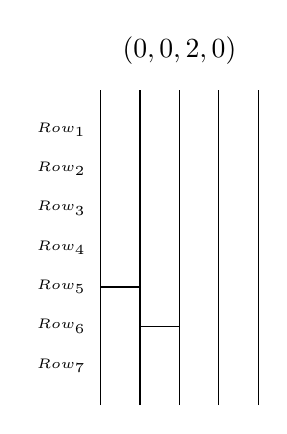
\begin{tikzpicture}
      \node at (1, 4.5){$(0,0,2,0)$};
      \draw(0, 0) to (0, 4);
        \draw(0, 1.5) to (0.5, 1.5);
      \draw(0.5, 0) to (.5, 4);
      \draw(1, 0) to (1, 4);
        \draw(0.5, 1) to (1, 1);
      \draw(1.5, 0) to (1.5, 4);
      \draw(2, 0) to (2, 4);

      \node at(-0.5, 3.5){\tiny{$Row_{1}$}};
      \node at(-0.5, 3.0){\tiny{$Row_{2}$}};
      \node at(-0.5, 2.5){\tiny{$Row_{3}$}};
      \node at(-0.5, 2.0){\tiny{$Row_{4}$}};
      \node at(-0.5, 1.5){\tiny{$Row_{5}$}};
      \node at(-0.5, 1.0){\tiny{$Row_{6}$}};
      \node at(-0.5, 0.5){\tiny{$Row_{7}$}};
    \end{tikzpicture}
  \end{minipage}


   \begin{minipage}{.3\textwidth}
    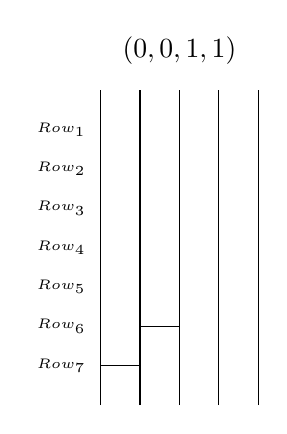
\begin{tikzpicture}
      \node at (1, 4.5){$(0,0,1,1)$};
      \draw(0, 0) to (0, 4);
        \draw(0, 0.5) to (0.5, 0.5);
      \draw(0.5, 0) to (.5, 4);
      \draw(1, 0) to (1, 4);
        \draw(0.5, 1) to (1, 1);
      \draw(1.5, 0) to (1.5, 4);
      \draw(2, 0) to (2, 4);
      
      \node at(-0.5, 3.5){\tiny{$Row_{1}$}};
      \node at(-0.5, 3.0){\tiny{$Row_{2}$}};
      \node at(-0.5, 2.5){\tiny{$Row_{3}$}};
      \node at(-0.5, 2.0){\tiny{$Row_{4}$}};
      \node at(-0.5, 1.5){\tiny{$Row_{5}$}};
      \node at(-0.5, 1.0){\tiny{$Row_{6}$}};
      \node at(-0.5, 0.5){\tiny{$Row_{7}$}};
    \end{tikzpicture}
  \end{minipage}
   \begin{minipage}{.3\textwidth}
    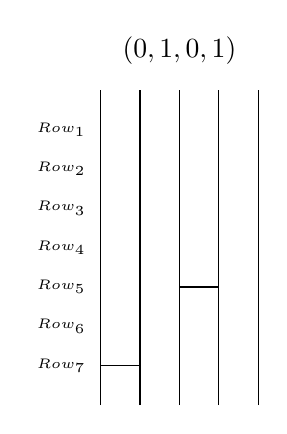
\begin{tikzpicture}
      \node at (1, 4.5){$(0,1,0,1)$};
      \draw(0, 0) to (0, 4);
        \draw(0, 0.5) to (0.5, 0.5);
      \draw(0.5, 0) to (.5, 4);
      \draw(1, 0) to (1, 4);
        \draw(1, 1.5) to (1.5, 1.5);
      \draw(1.5, 0) to (1.5, 4);
      \draw(2, 0) to (2, 4);
      
      \node at(-0.5, 3.5){\tiny{$Row_{1}$}};
      \node at(-0.5, 3.0){\tiny{$Row_{2}$}};
      \node at(-0.5, 2.5){\tiny{$Row_{3}$}};
      \node at(-0.5, 2.0){\tiny{$Row_{4}$}};
      \node at(-0.5, 1.5){\tiny{$Row_{5}$}};
      \node at(-0.5, 1.0){\tiny{$Row_{6}$}};
      \node at(-0.5, 0.5){\tiny{$Row_{7}$}};
    \end{tikzpicture}
  \end{minipage}
   \begin{minipage}{.3\textwidth}
    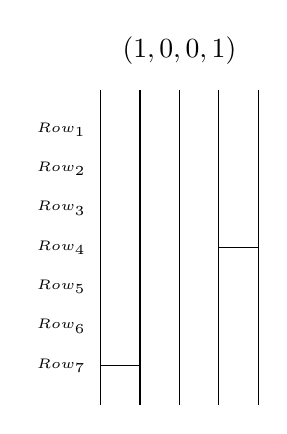
\begin{tikzpicture}
      \node at (1, 4.5){$(1,0,0,1)$};
      \draw(0, 0) to (0, 4);
        \draw(0, 0.5) to (0.5, 0.5);
      \draw(0.5, 0) to (.5, 4);
      \draw(1, 0) to (1, 4);
        \draw(1.5, 2) to (2, 2);
      \draw(1.5, 0) to (1.5, 4);
      \draw(2, 0) to (2, 4);
      
      \node at(-0.5, 3.5){\tiny{$Row_{1}$}};
      \node at(-0.5, 3.0){\tiny{$Row_{2}$}};
      \node at(-0.5, 2.5){\tiny{$Row_{3}$}};
      \node at(-0.5, 2.0){\tiny{$Row_{4}$}};
      \node at(-0.5, 1.5){\tiny{$Row_{5}$}};
      \node at(-0.5, 1.0){\tiny{$Row_{6}$}};
      \node at(-0.5, 0.5){\tiny{$Row_{7}$}};
    \end{tikzpicture}
  \end{minipage}




  \caption{Listing $L_{5,2}$ with Walsh's Gray code on bar vector $g$. Ladders are read left to right, top to bottom. $g$ is listed above 
  each ladder.}
  \label{Fig:LnK}
 \end{figure}
 \pagebreak

 Walsh provides a loop free algorithm to list $g$ in Gray code order~\cite{A41}. His algorithm provides the next 
 instance of $g$ in $O(1)$ time by providing the $x$ and $w$ indices in $O(1)$ time. We use Walsh's algorithm 
 to provide the $x$ and $w$ value in order to list the next canonical ladder in $L_{n+1, k}$. Walsh refers to $x$ as 
 pivot one and $w$ as pivot two. We note that $x>w$. We also note that $g_{x}$ is incremented or decremented 
 before $g_{w}$ is decremented or incremented. In Algorithm~\ref{Alg:NextLadderLnK}, 
 termed {\sc NextLadderNK}, we list the next canonical ladder using the pivots $x$ and $w$ provided by Walsh's algorithm. The initial conditions 
 of {\sc NextLadderNK} are the following. Let $x$ be pivot one returned from Walsh's algorithm. Let $w$ be pivot two 
 returned from Walsh's algorithm. Let $CL$ be a canonical ladder with $n+1$ lines and $k$ bars. Let $increment$ be a Boolean 
 variable set to \textbf{true} if the pivot one is incremented and pivot two is decremented, else $increment$ is set to \textbf{false}. 
\begin{algorithm}
  \begin{algorithmic}[1]
    \Function{NextLadderNK}{$x$, $w$, $CL$, $increment$}
      \If{$increment=$\textbf{true}} \Comment{Add bar to ass. diag. $(n+x)-1$}
        \State $(row_{x}, column_{x}) \gets  ((n+x-1)-g_{x}, (n+1-x)-g_{x})$
        \State $(row_{w}, column_{w}) \gets  ((n+w)-g_{w}, (n+1-w)-g_{w}+1)$
        \State $CL[row_{x}][column_{x}] \gets 1$
        \State $CL[row_{w}][column_{w}] \gets 0$
      \Else \Comment{Remove bar from ass. diag. $(n+x)-1$}
        \State $(row_{w}, column_{w}) \gets  ((n+w-1)-g_{w}, (n+1-w)-g_{w})$
        \State $(row_{x}, column_{x}) \gets  ((n+x)-g_{x}, (n+1-x)-g_{x}+1)$
        \State $CL[row_{x}][column_{x}] \gets 0$
        \State $CL[row_{w}][column_{w}] \gets 1$
      \EndIf
   \EndFunction
  \end{algorithmic}
  \caption{Algorithm to list the next ladder in $L_{n+1, k}$}
  \label{Alg:NextLadderLnK}
\end{algorithm}

\begin{corollary}
  {\sc NextLadderNK} produces the next ladder in $L_{n+1, k}$ in $O(1)$ time.
\end{corollary}
\begin{proof}
  From Walsh's paper, we know that we can attain the first and second pivot in $O(1)$ time. We use these pivots, $x$ and $w$, to calculate the 
  row and column for the coordinates of the bar to add, and the coordinates of the bar to remove, in $O(1)$ time. 
\end{proof}

We use {\sc NextLadderNK} as a subroutine in Algorithm~\ref{Alg:ListLNK}, termed {\sc ListLNK}, which lists $L_{n,k}$ 
in Gray code order. Let $k$ be 
the number of bars. Let $n$ be the number of lines in $CL$. 
Let $g$ be initialized to the lexicographically largest composition; $(k,0, \dots, 0)$. Let $m$ be the bound on $g$. 
We note that $g$ and $m$ are of order $n-1$.
Let $CL$ be the canonical ladder data structure initialized as the lexicographically largest ladder. 
Let $p1$ and $p2$ be pivot one and pivot two respectively. 
Let $increment$ be a Boolean set to \textbf{true} if $p1$ is to be incremented and $p2$ is to be decremented, 
else $increment$ is set to \textbf{false}. 
\begin{algorithm}
  \begin{algorithmic}[1]
    \Function{ListLNK}{$g$, $m$, $CL$, $k$}
      \State {\sc Print}($CL$)
      \State $increment \gets$ \textbf{true}
      \While{$g_{1}<m_{1}$ \textbf{and} $g_{1}< k-(g_{2}+ \dots +g_{n-1})$}\Comment{while not at last composition}
        \State $(p1,p2) \gets ${\sc Walsh}$(g,m, \dots)$
        \If{$(g_{p1+1},+ \dots ,+g_{n-1})$ is even} $p1 \gets p1+1$, $p2 \gets p2-1$
        \Else $\: p1 \gets p1-1$, $p2 \gets p2+1$
        \EndIf

        \If{$g_{1}>m_{1}$ \textbf{or} $g_{1}>k-(g_{2}+ \dots +g_{n-1})$}\Comment{surpassed last composition}
          \State $g_{1} \gets g_{1}-1$
          \State $g_{p1} \gets g_{p1}+1$
          \State \textbf{return}
        \EndIf
        \If{$(g_{p1+1}+ \dots +g_{n-1})$ is even} $increment \gets $ \textbf{true}
        \Else $:\ increment \gets $ \textbf{false}
        \EndIf
        \State {\sc NextLadderNK}$(p1, p2, CL, increment)$
        \State {\sc Print}($CL$)
      \EndWhile
    \EndFunction
  \end{algorithmic}
  \caption{Algorithm for listing $L{n,k}$}
  \label{Alg:ListLNK}
\end{algorithm} 

By applying Walsh's algorithm, which returns $p1$ and $p2$ in $O(1)$ time, we produce $L_{n,k}$ in constant amortized time per ladder. 
We note that line $6$ of the algorithm determines the parity of the suffix; Walsh demonstrates that the parity 
of the suffix can be determined in $O(1)$ time by maintaining a number of auxiliary data structures~\cite{A41}.  


\section{Listing $L_{n}$ by $k$ bars}
In the previous section, we applied Walsh's Gray code for listing $L_{n,k}$. In this section, we further modify Walsh's Gray code 
to list $L_{n}$ by way of listing $L_{n,0} \dots L_{n,k} \dots L_{n, {n \choose 2}}$ in Gray code order. 
To reiterate, we list $L_{n}$ by way of $L_{n,k}$ by first listing all ladders with exactly $k$ bars before we list the first ladder with $k+1$ bars. In Figure~\ref{Fig:LnByk} we show the 
listing of $L_{4}$ by listing $L_{4,0} \dots L_{4, k} \dots L_{4, 6}$.\par 

\begin{figure}[htp]
  \centering
\resizebox{!}{.6\textheight}{
  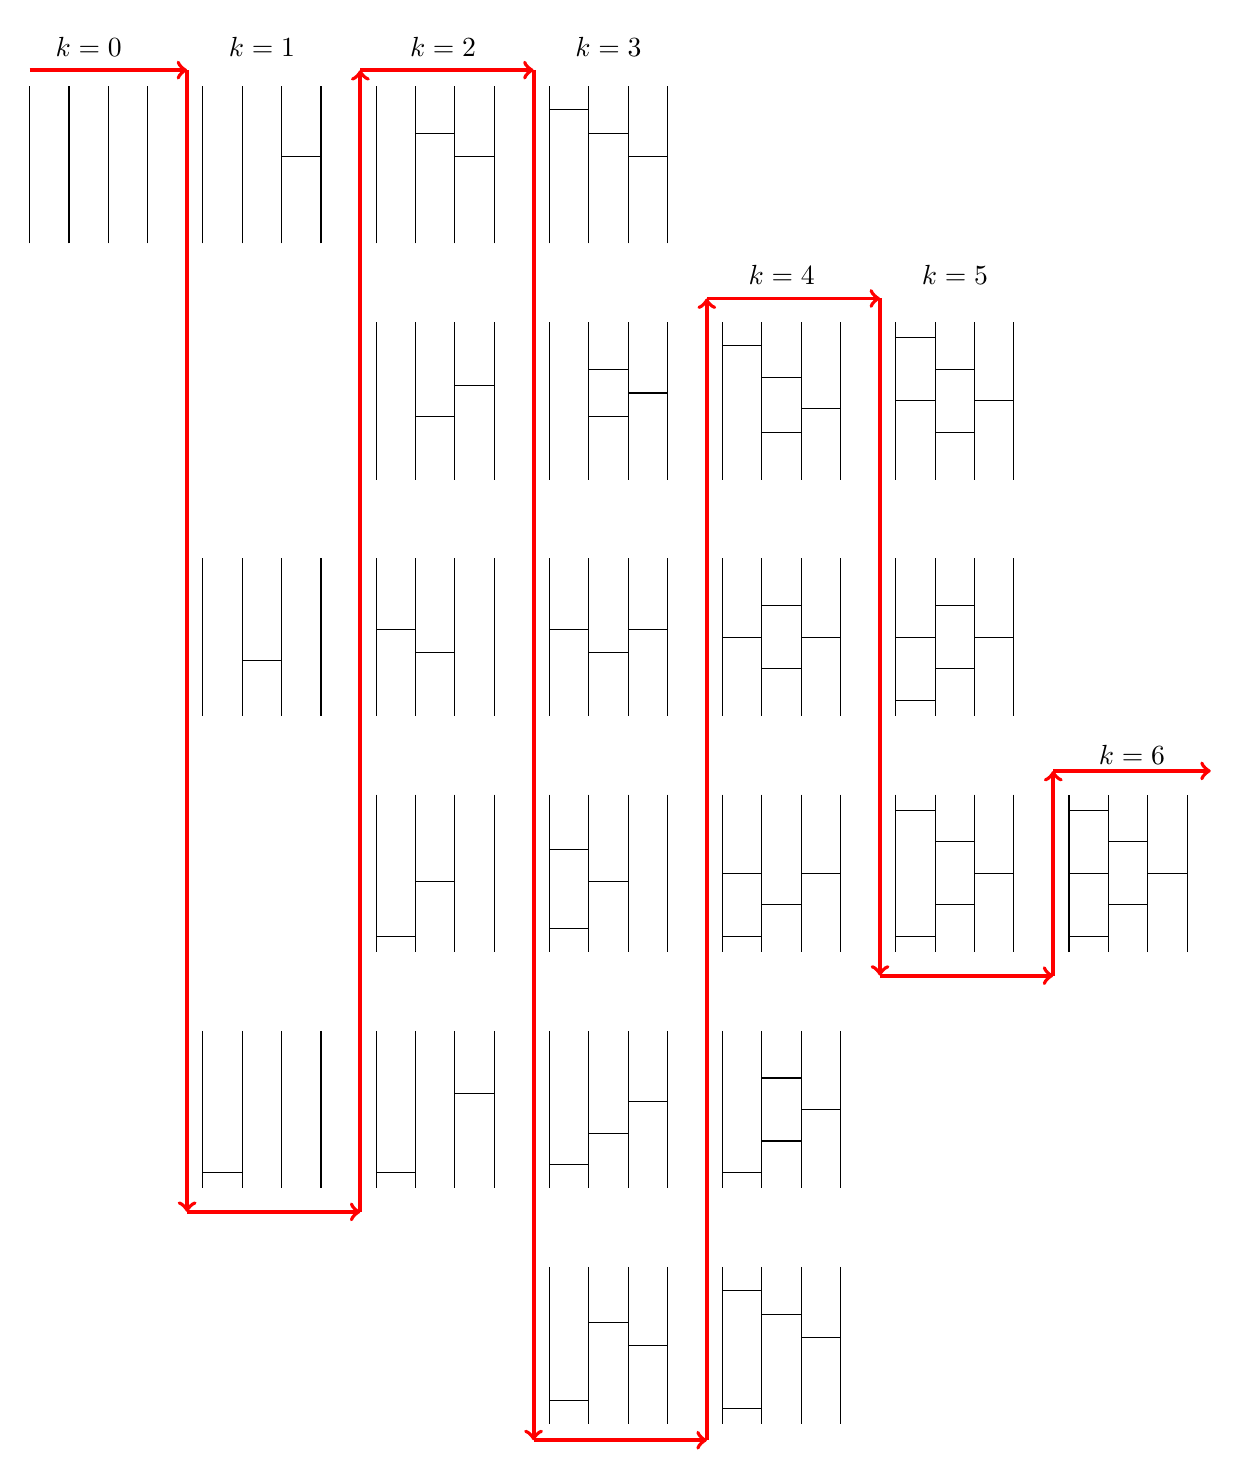
\begin{tikzpicture}
            \node at(0.75, 2.5){$k=0$};
             %%k = 0
                \draw(0, 0) to (0, 2);
                \draw(0.5, 0) to (0.5, 2);
                \draw(1, 0) to (1, 2);
                \draw(1.5, 0) to (1.5, 2);
                \draw[line width=.5mm, color=red, ->](0, 2.2) to (2, 2.2);
            %%k = 1    
                \draw[line width=.5mm, color=red, ->](2, 2.2) to (2, -12.3);
                \node at (2.95, 2.5){$k=1$};
                \draw(2.2, 0) to (2.2, 2);
                \draw(2.7, 0) to (2.7, 2);
                \draw(3.2, 0) to (3.2, 2);
                    \draw(3.2, 1.1) to (3.7, 1.1);
                \draw(3.7, 0) to (3.7, 2);
               
                
                \draw(2.2, -4) to (2.2, -6);
                \draw(2.7, -4) to (2.7, -6);
                    \draw(2.7, -5.3) to (3.2, -5.3);
                \draw(3.2, -4) to (3.2, -6);
                    %\draw(2.2, -5.8) to (2.7, -5.8);
                \draw(3.7, -4) to (3.7, -6);
                
                 
                \draw(2.2, -10) to (2.2, -12);
                    \draw(2.2, -11.8) to (2.7, -11.8);
                \draw(2.7, -10) to (2.7, -12);
                    
                \draw(3.2, -10) to (3.2, -12);
                \draw(3.7, -10) to (3.7, -12);
                
               \draw[line width=.5mm, color=red, ->](2, -12.3) to (4.2, -12.3);

                
            %%k=2
            \draw[line width=.5mm, color=red, ->](4.2, -12.3) to (4.2, 2.2);
                \node at(5.25, 2.5){$k=2$};
                \draw(4.4, 0) to (4.4, 2);
                \draw(4.9, 0) to (4.9, 2);
                    \draw(4.9, 1.4) to (5.4, 1.4);
                \draw(5.4, 0) to (5.4, 2);
                    \draw(5.4, 1.1) to (5.9, 1.1);
                \draw(5.9, 0) to (5.9, 2);
                
                \draw(4.4, -1) to (4.4, -3);
                \draw(4.9, -1) to (4.9, -3);
                    \draw(4.9, -2.2) to (5.4, -2.2);
                \draw(5.4, -1) to (5.4, -3);
                  \draw(5.4, -1.8) to (5.9, -1.8); 
                \draw(5.9, -1) to (5.9, -3);
                
                \draw(4.4, -4) to (4.4, -6);
                \draw(4.9, -4) to (4.9, -6);
                    \draw(4.9, -5.2) to (5.4, -5.2);
                    \draw(4.4, -4.9) to (4.9, -4.9);
                \draw(5.4, -4) to (5.4, -6);
                \draw(5.9, -4) to (5.9, -6);
                
                \draw(4.4, -7) to (4.4, -9);
                    \draw(4.4, -8.8) to (4.9, -8.8);
                \draw(4.9, -7) to (4.9, -9);
                    \draw(4.9, -8.1) to (5.4, -8.1);
                \draw(5.4, -7) to (5.4, -9);
                \draw(5.9, -7) to (5.9, -9);
                
                 \draw(4.4, -10) to (4.4, -12);
                    \draw(4.4, -11.8) to (4.9, -11.8);
                \draw(4.9, -10) to (4.9, -12);
                \draw(5.4, -10) to (5.4, -12);
                    \draw(5.4,-10.8) to (5.9, -10.8);
                \draw(5.9, -10) to (5.9, -12);
                
                \draw[line width=.5mm, color=red, ->](4.2, 2.2) to (6.4, 2.2);

                
            %%k=3
            \draw[line width=.5mm, color=red, ->](6.4, 2.2) to (6.4, -15.2);
                \node at(7.35, 2.5){$k=3$};
                \draw(6.6, 0) to (6.6, 2);
                    \draw(6.6, 1.7) to (7.1, 1.7);
                \draw(7.1, 0) to (7.1, 2);
                    \draw(7.1, 1.4) to (7.6, 1.4);
                \draw(7.6, 0) to (7.6, 2);
                    \draw(7.6, 1.1) to (8.1, 1.1);
                \draw(8.1, 0) to (8.1, 2);
                
                \draw(6.6, -1) to (6.6, -3);
                \draw(7.1, -1) to (7.1, -3);
                    \draw(7.1, -2.2) to (7.6, -2.2);
                    \draw(7.1, -1.6) to (7.6, -1.6);
                \draw(7.6, -1) to (7.6, -3);
                    \draw(7.6, -1.9) to (8.1, -1.9);
                \draw(8.1, -1) to (8.1, -3);


                \draw(6.6, -4) to (6.6, -6);
                    \draw(6.6, -4.9) to (7.1, -4.9);
                \draw(7.1, -4) to (7.1, -6);
                    \draw(7.1, -5.2) to (7.6, -5.2);
                \draw(7.6, -4) to (7.6, -6);
                    \draw(7.6, -4.9) to (8.1, -4.9);
                \draw(8.1, -4) to (8.1, -6);
                
                \draw(6.6, -7) to (6.6, -9);
                    \draw(6.6, -8.7) to (7.1, -8.7);
                    \draw(6.6, -7.7) to (7.1, -7.7);
                \draw(7.1, -7) to (7.1, -9);
                    \draw(7.1, -8.1) to (7.6, -8.1);
                \draw(7.6, -7) to (7.6, -9);
                \draw(8.1, -7) to (8.1, -9);
                
                \draw(6.6, -10) to (6.6, -12);
                    \draw(6.6, -11.7) to (7.1, -11.7);
                \draw(7.1, -10) to (7.1, -12);
                    \draw(7.1, -11.3) to (7.6, -11.3); 
                \draw(7.6, -10) to (7.6, -12);
                    \draw(7.6, -10.9) to (8.1, -10.9);
                \draw(8.1, -10) to (8.1, -12);
                
                \draw(6.6, -13) to (6.6, -15);
                    \draw(6.6, -14.7) to (7.1, -14.7);
                \draw(7.1, -13) to (7.1, -15);
                    \draw(7.1, -13.7) to (7.6, -13.7);
                \draw(7.6, -13) to (7.6, -15);
                    \draw(7.6, -14) to (8.1, -14);
                \draw(8.1, -13) to (8.1, -15);
                
                \draw[->, color=red, line width = 0.5mm](6.4, -15.2) to (8.6, -15.2);
            
            %%k=4
                \node at(9.55, -.4){$k=4$};
                \draw(8.8, -1) to (8.8, -3);
                    \draw(8.8, -1.3) to (9.3, -1.3);
                \draw(9.3, -1) to (9.3, -3);
                    \draw(9.3, -1.7) to (9.8, -1.7);
                    \draw(9.3, -2.4) to (9.8, -2.4);
                \draw(9.8, -1) to (9.8, -3);
                    \draw(9.8, -2.1) to (10.3, -2.1);
                \draw(10.3, -1) to (10.3, -3);


                \draw(8.8, -4) to (8.8, -6);
                    \draw(8.8, -5) to (9.3, -5);
                \draw(9.3, -4) to (9.3, -6);
                    \draw(9.3, -4.6) to (9.8, -4.6);
                    \draw(9.3, -5.4) to (9.8, -5.4);
                \draw(9.8, -4) to (9.8, -6);
                    \draw(9.8, -5) to (10.3, -5);s
                \draw(10.3, -4) to (10.3, -6);
                
                \draw(8.8, -7) to (8.8, -9);
                    \draw(8.8, -8.8) to (9.3, -8.8);
                    \draw(8.8, -8.0) to (9.3, -8.0);
                \draw(9.3, -7) to (9.3, -9);
                    \draw(9.3, -8.4) to (9.8, -8.4);
                \draw(9.8, -7) to (9.8, -9);
                    \draw(9.8, -8.0) to (10.3, -8.0);
                \draw(10.3, -7) to (10.3, -9);
                
                \draw(8.8, -10) to (8.8, -12);
                    \draw(8.8, -11.8) to (9.3, -11.8);
                \draw(9.3, -10) to (9.3, -12);
                    \draw(9.3, -11.4) to (9.8, -11.4);
                    \draw(9.3, -10.6) to (9.8, -10.6);
                \draw(9.8, -10) to (9.8, -12);
                    \draw(9.8, -11)to(10.3, -11);
                \draw(10.3, -10) to (10.3, -12);
                
                \draw(8.8, -13) to (8.8, -15);
                    \draw(8.8, -14.8) to (9.3, -14.8);
                    \draw(8.8, -13.3) to (9.3, -13.3);
                \draw(9.3, -13) to (9.3, -15);
                    \draw(9.3, -13.6) to (9.8, -13.6);
                \draw(9.8, -13) to (9.8, -15);
                    \draw(9.8, -13.9) to (10.3, -13.9);
                \draw(10.3, -13) to (10.3, -15);
                
                
                \draw[->, color=red, line width = 0.5mm](8.6, -15.2) to (8.6, -.7);
            %%k = 5
                 \draw[->, color=red, line width = 0.5mm](8.6, -.7) to (10.8, -.7);
                 \node at(11.75, -.4){$k=5$};
                 \draw(11, -1) to (11, -3);
                    \draw(11, -1.2) to (11.5, -1.2);
                    \draw(11, -2) to (11.5, -2);
                 \draw(11.5, -1) to (11.5, -3);
                    \draw(11.5, -1.6) to (12, -1.6);
                    \draw(11.5, -2.4) to (12, -2.4);
                 \draw(12, -1) to (12, -3);
                    \draw(12, -2) to (12.5, -2);
                 \draw(12.5, -1) to (12.5, -3);
                 
                 \draw(11, -4) to (11, -6);
                    \draw(11, -5) to (11.5, -5);
                    \draw(11, -5.8) to (11.5, -5.8);
                 \draw(11.5, -4) to (11.5, -6);
                    \draw(11.5, -5.4) to (12, -5.4);
                    \draw(11.5, -4.6) to (12, -4.6);
                 \draw(12, -4) to (12, -6);
                    \draw(12, -5) to (12.5, -5);
                 \draw(12.5, -4) to (12.5, -6);


                 \draw(11, -7) to (11, -9);
                    \draw(11, -7.2) to (11.5, -7.2);
                    \draw(11, -8.8) to (11.5, -8.8);
                 \draw(11.5, -7) to (11.5, -9);
                    \draw(11.5, -7.6) to (12, -7.6);
                    \draw(11.5, -8.4) to (12, -8.4);
                 \draw(12, -7) to (12, -9);
                    \draw(12, -8) to (12.5, -8);
                 \draw(12.5, -7) to (12.5, -9);
                 
                \draw[->, color=red, line width = 0.5mm](10.8, -.7) to(10.8, -9.3);
                
            %%k=6
            \draw[->, color=red, line width = 0.5mm](10.8, -9.3) to(13, -9.3);
            \node at(14, -6.5){$k=6$};
            \draw(13.2, -9) to (13.2, -7);
                \draw(13.2, -7.2) to (13.7, -7.2);
                \draw(13.2, -8) to (13.7, -8);
                \draw(13.2, -8.8) to (13.7, -8.8);
            \draw(13.7, -9) to (13.7, -7);
                \draw(13.7, -7.6) to (14.2, -7.6);
                \draw(13.7, -8.4) to (14.2, -8.4);
            \draw(14.2, -9) to (14.2, -7);
                \draw(14.2, -8) to (14.7, -8);
            \draw(14.7, -9) to (14.7, -7);
            \draw[->, color=red, line width=0.5mm](13, -9.3) to (13, -6.7);
            \draw[->, color=red, line width=0.5mm](13, -6.7) to (15, -6.7);
            \end{tikzpicture}}
           
      \caption{Listing of $L_{4}$ by $k$ bars. For each $k$, successive ladders differ by the relocation of a bar. Transitioning from the last ladder in $L_{n,k}$ to the first ladder in $L_{n,k+1}$ requires the addition of a bar.}
      \label{Fig:LnByk}
\end{figure}


We previously defined the lexicographically largest ladder as the ladder such 
the associated diagonal of any element $y>w$, the number of bars in $y's$ diagonal is the $min(m_{(n+1-y)+1}, k-\text{the number of bars along the associated diagonals of } n+1,n,\dots,y+1)$. 
We now define the \emph{terminating ladder} as follows - let the 
first $k-1$ bars compose the sub-ladder along the associated diagonals from $3 \dots y \dots n$; this sub-ladder is the 
lexicographically largest sub-ladder. Bar $k$ occupies the associated diagonal of $2$. For an example of the terminating ladder 
for $L_{5, 6}$, please refer to Figure~\ref{Fig:TerminatingLadder}. We describe the corresponding $g$, termed 
the \emph{terminating composition $g$}, as $(k-1, 0, \dots, 1)$. 
\begin{figure}[h]
  \centering 
  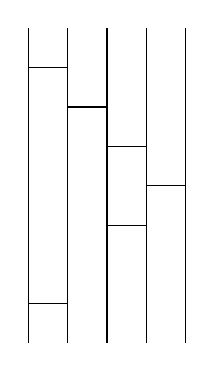
\begin{tikzpicture}
  \draw(0, 0) to (0, 4);
    \draw(0, 3.5) to (0.5, 3.5);
    \draw(0, 0.5) to (0.5, 0.5);
  \draw(0.5, 0) to (0.5, 4);
    \draw(0.5, 3) to (1, 3);
  \draw(1, 0) to (1, 4);
    \draw(1, 2.5) to (1.5, 2.5);
    \draw(1, 1.5) to (1.5, 1.5);
  \draw(1.5, 0) to (1.5, 4);
    \draw(1.5, 2) to (2, 2);
  \draw(2, 0) to (2, 4);
  \end{tikzpicture}
  \caption{The terminating ladder for $L_{5,6}$}
  \label{Fig:TerminatingLadder}
\end{figure}

In order to list $L_{n}$ by way of $L_{n,k}$, we use Walsh's Gray code on composition $g$ when $k$ is odd. Recall, that 
when $k$ is odd we start at the lexicographically largest $g$ and end at the terminating $g$. Therefore, our description of 
listing $L_{n,k}$ by way of $g$ in the previous section still holds for odd values of $k$. However, when $k$ is even we 
start with the terminating $g$ and we have to work backwards so to speak, ending at the lexicographically largest $g$.
We assume by providing the inverse of Walsh's Gray code, we can list $g$ for even values of $k$. 
We provide two conjectures, Conjecture~\ref{Conjecture:ReverseOrdering} and Conjecture~\ref{Conjecture:ReverseWalsh},
that could allow for the algorithmic implementation of the reverse ordering of Walsh's Gray code. If 
Conjecture~\ref{Conjecture:ReverseOrdering} is true, we have a sufficient condition for Conjecture~\ref{Conjecture:ReverseWalsh} being true. 
\begin{conjecture}
  We refer to $x$ as $p1$ and $w$ as $p2$.
  When listing $g$ in reverse order, we list $g$ as follows-starting from $g_{2}$, 
  scan left to right until you find a $g_{x}$ not at its last value such that if $(g_{x+1}, + \dots + ,g_{n})$ is odd and there exists some minimum $1 \leq w \leq x-1$ 
  such that $g_{w}$ that is not at its minimum value then increment $g_{p1}$ and decrement $g_{p2}$. If $(g_{x+1} + \dots +g_{n})$ is even and there 
  exists some minimum $1 \leq w \leq x-1$ such that $g_{w}$ is not at its maximum value, decrement $g_{p1}$ and increment $g_{p2}$. 
  \label{Conjecture:ReverseOrdering}
\end{conjecture}
Under the assumption Conjecture~\ref{Conjecture:ReverseOrdering} is true, we state Conjecture~\ref{Conjecture:ReverseWalsh}.
\begin{conjecture}
  Assuming ~\ref{Conjecture:ReverseOrdering} is true, by starting with the terminating composition of $g$ and ending at the 
  lexicographically largest composition of $g$, we  
  can implement the inverse of Walsh's algorithm for listing $g$ in reverse ordering with $O(1)$ time per instance of $g$. 
  \label{Conjecture:ReverseWalsh}
\end{conjecture}
In Figure~\ref{Fig:ReverseOrdering}, we apply Conjecture~\ref{Conjecture:ReverseOrdering}
to provide the Gray code for the composition $g$ on $S_{5,4}$ in reverse order. We also give
 the Gray code for the permutations when we map $g$ to the associated diagonals of the canonical ladder. 
We start with the terminating composition of $g$ 
and the permutation corresponding to the terminating ladder. We end at the lexicographically largest composition and the permutation corresponding 
to the lexicographically largest canonical ladder. The pivots, $p1$ and $p2$ are bolded; the pivots bolded in composition $i$ indicate which 
two values in composition $i$ will be incremented and decremented in order to transition to composition $i+1$. Recall, that the first pivot $p1$ is greater 
than the second pivot $p2$.\pagebreak
\begin{figure}[ht]
  \centering 
  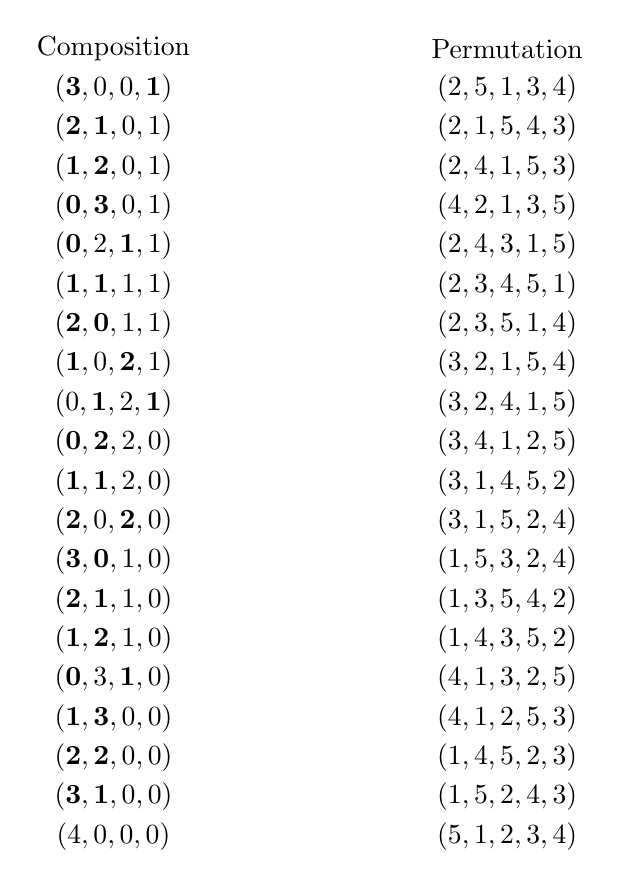
\begin{tikzpicture}
    \node at (0, 50){Composition};                       \node at (5, 50){{Permutation}};
    \node at (0, 49.5){$(\mathbf{3},0,0,\mathbf{1})$};   \node at (5, 49.5){$(2,5,1,3,4)$};  
    \node at (0, 49){$(\mathbf{2},\mathbf{1},0,1)$};     \node at (5, 49){$(2,1,5,4,3)$};
    \node at (0, 48.5){$(\mathbf{1},\mathbf{2},0,1)$};   \node at (5, 48.5){$(2,4,1,5,3)$};
    \node at (0, 48){$(\mathbf{0},\mathbf{3},0,1)$};     \node at (5, 48){$(4,2,1,3,5)$};
    \node at (0, 47.5){$(\mathbf{0},2,\mathbf{1},1)$};   \node at (5, 47.5){$(2,4,3,1,5)$};
    \node at (0, 47){$(\mathbf{1},\mathbf{1},1,1)$};     \node at (5, 47){$(2,3,4,5,1)$};
    \node at (0, 46.5){$(\mathbf{2},\mathbf{0},1,1)$};   \node at (5, 46.5){$(2,3,5,1,4)$};
    \node at (0, 46){$(\mathbf{1},0,\mathbf{2},1)$};     \node at (5, 46){$(3,2,1,5,4)$};

   \node at (0, 45.5){$(0,\mathbf{1},2,\mathbf{1})$};   \node at (5, 45.5){$(3,2,4,1,5)$};

   \node at (0, 45){$(\mathbf{0},\mathbf{2},2,0)$};     \node at (5, 45){$(3,4,1,2,5)$};

   \node at (0, 44.5){$(\mathbf{1},\mathbf{1},2,0)$};   \node at (5, 44.5){$(3,1,4,5,2)$};

   \node at (0, 44){$(\mathbf{2},0,\mathbf{2},0)$};     \node at (5, 44){$(3,1,5,2,4)$};

   \node at (0, 43.5){$(\mathbf{3},\mathbf{0},1,0)$};   \node at (5, 43.5){$(1,5,3,2,4)$};

   \node at (0, 43){$(\mathbf{2},\mathbf{1},1,0)$};     \node at (5, 43){$(1,3,5,4,2)$};

   \node at (0, 42.5){$(\mathbf{1},\mathbf{2},1,0)$};   \node at (5, 42.5){$(1,4,3,5,2)$};

   \node at (0, 42){$(\mathbf{0},3,\mathbf{1},0)$};     \node at (5, 42){$(4,1,3,2,5)$};

   \node at (0, 41.5){$(\mathbf{1},\mathbf{3},0,0)$};   \node at (5, 41.5){$(4,1,2,5,3)$};

   \node at (0, 41){$(\mathbf{2},\mathbf{2},0,0)$};     \node at (5, 41){$(1,4,5,2,3)$};

   \node at (0, 40.5){$(\mathbf{3},\mathbf{1},0,0)$};   \node at (5, 40.5){$(1,5,2,4,3)$};

   \node at (0, 40){$(4,0,0,0)$};                       \node at (5, 40){$(5,1,2,3,4)$};

   



   
  \end{tikzpicture}
  \caption{Ordering of $g$ based on Conjecture~\ref{Conjecture:ReverseOrdering} and the ordering of permutations corresponding to $L_{5,4}$ when 
  $g$ is mapped to the associated diagonals.}
  \label{Fig:ReverseOrdering}
\end{figure}
\pagebreak

We use Conjecture~\ref{Conjecture:ReverseOrdering} and Conjecture~\ref{Conjecture:ReverseWalsh} to create Algorithm~\ref{Alg:ListLNKReverse}, 
termed {\sc ListLNKReverse} to provide a reverse listing of all ladders of order $n$ with $k$ bars in Gray code order. 
Let $k$ be the number of bars. Let $n$ be the number of lines in $CL$. 
Let $g$ be initialized to the terminating composition; $(k-1,0, \dots, 1)$. Let $m$ be the bound on $g$. 
We note that $g$ and $m$ are of order $n-1$.
Let $CL$ be the canonical ladder data structure initialized as the lexicographically largest ladder. 
Let $p1$ and $p2$ be pivot one and pivot two respectively. 
Let $increment$ be a Boolean set to \textbf{true} if $p1$ is to be incremented and $p2$ is to be decremented, 
else $increment$ is set to \textbf{false}. Let {\sc ReverseWalsh} be the hypothetical implementation of the inverse 
of Walsh's algorithm, which is used as a subroutine to 
return $p1$ and $p2$ in such a way that $g$ can be listed in reverse order. 

\begin{algorithm}
  \begin{algorithmic}[1]
    \Function{ListLNKReverse}{$g$, $m$, $CL$, $k$}
      \State {\sc Print}($CL$)
      \State $increment \gets$ \textbf{true}
      \While{$g_{1}<m_{1}$ \textbf{and} $g_{1}< k-(g_{2}+ \dots +g_{n-1})$}\Comment{while not at lex. largest composition}
        \State $(p1,p2) \gets ${\sc ReverseWalsh}$(g,m, \dots)$\Comment{Assuming Conjecture~\ref{Conjecture:ReverseWalsh} is correct}
        \If{$(g_{p1+1},+ \dots ,+g_{n-1})$ is odd} $p1 \gets p1+1$, $p2 \gets p2-1$
        \Else $\: p1 \gets p1-1$, $p2 \gets p2+1$
        \EndIf

        \If{$g_{1}>m_{1}$ \textbf{or} $g_{1}>k-(g_{2} + \dots + g_{n-1})$}\Comment{surpassed lex. largest composition}
          \State $g_{1} \gets g_{1}-1$
          \State $g_{2} \gets g2_{+1}$
          \State \textbf{return}
        \EndIf
        \If{$(g_{p1+1},+ \dots ,+g_{n-1})$ is odd} $increment \gets $ \textbf{true} \Comment{Assuming Conjecture~\ref{Conjecture:ReverseOrdering} is correct}
        \Else $:\ increment \gets $ \textbf{false}
        \EndIf
        \State {\sc NextLadderNK}$(p1, p2, CL, increment)$
        \State {\sc Print}($CL$)
      \EndWhile
    \EndFunction
  \end{algorithmic}
  \caption{Algorithm for listing $L{n,k}$ starting from the terminating ladder and ending at the lexicographically largest ladder.}
  \label{Alg:ListLNKReverse}
\end{algorithm} 

Assuming we implement the inverse of Walsh's algorithm, we would be able to list $L_{n,k}$  in constant amortized time in 
the reverse ordering of Walsh's Gray code order.\par
When we list $L_{n}$, if $k$ is odd, the first ladder listed in $L_{n,k}$ is the lexicographically 
largest ladder and the last ladder listed is the terminating ladder. If $k$ is even, 
the first ladder listed in $L_{n,k}$ is the terminating ladder and the last ladder listed is the lexicographically largest ladder.
When listing $L_{n}$, we use the terminating ladder and the lexicographically largest ladder as the transitioning 
ladders between $L_{n,k}$ and $L_{n,k+1}$. When we reach the last ladder in $L_{n,k}$, we add a bar 
to said ladder and transition to the first ladder of $L_{n, k+1}$. We refer to this bar as the \emph{incrementing bar}. 
To calculate the coordinates of the incrementing bar when transitioning 
from $L_{n,k}$ to $L_{n,k+1}$, we scan $g$ from left to right to find the smallest $x$ 
value such that $g_{x}$ is not at its maximum value. We then use the same formula for adding a bar found in Equation~\ref{GetCoordinates3}, 
except we replace $n$ with $n-1$ seeing as $g$ is of order $n-1$ when mapping to canonical ladders with $n$ lines. If the last ladder 
of $L_{n,k}$ is a terminating ladder, when we add the incrementing bar, the first ladder of $L_{n,k+1}$ is also a terminating ladder. If the 
las ladder of $L_{n,k}$ is a lexicographically largest ladder, when we add the incrementing bar, the first ladder of $L_{n,k+1}$ is also a 
lexicographically largest ladder.\par 
To transition from $L_{n, k}$ to $L_{n, k+1}$ we want to add the incrementing bar to the 
largest associated diagonal that has room for one more bar. We know that by mapping 
$g$ to the associated diagonals, we can use $m$ to determine the largest associated diagonal that has room for one more bar. 
Based on our mapping of $g$ to the associated diagonals, the smallest $x$ value in $g$ not at its $m_{x}$ value corresponds to the largest 
associated diagonal where we can add bar $k+1$. 
Let $MinX$ be a global variable that keeps track of the smallest $x$ value in $g$ that is not at its 
$m_{x}$ value. When we list $g$ for $L_{n,k}$, we update $MinX$ with every transition from $g^{i}$ to $g^{i+1}$ using Algorithm~\ref{Alg:UpdateMinX}.
Let $p1$ be pivot one returned by Walsh's Gray code, let $p2$ be pivot two returned by Walsh's Gray code, let $g$ be the current composition, 
 let $m$ be the upper bound on $g$, and let $MinX$ be the current smallest $x$ value such that $g_{x}$ is not at its $m_{x}$ bound.\pagebreak
\begin{algorithm}
  \begin{algorithmic}[1]
    \Function{UpdateMinX}{$p1$, $p2$, $g$, $m$}
      \If{$p1 < MinX$ \textbf{and} $g_{p1}<${\sc Min}$(m_{p1},k-(g_{p1+1}+ \dots +g_{n-1})$)}
        \State $MinX \gets p1$
      \EndIf 
      \If{$p2 < MinX$ \textbf{and} $g_{p2} <${\sc Min}$(m_{p2},k-(g_{p1+1}+ \dots +g_{n-1})$) }
        \State $MinX \gets p2$ 
      \EndIf 
      \If{$g_{MinX} =$ {\sc Min}$(m_{MinX},k-(g_{p1+1}+ \dots +g_{n-1}))$} 
        \If {$MinX != p1$} 
          \State $MinX \gets p1$
          \textbf{return}
        \EndIf
        \If{$MinX != p2$} 
          \State $MinX \gets p2$
          \textbf{return}
        \EndIf
      \EndIf
    \EndFunction
  \end{algorithmic}
  \caption{Algorithm for updating the minimum $x$ value such that $g_{x}<m_{x}$}
  \label{Alg:UpdateMinX}
\end{algorithm}
With {\sc UpdateMinX}, we are able to determine the row and column of the incrementing bar in $O(1)$ time. 
\emph{Due to the ordering of the algorithms and concepts in this chapter, our 
pseudocode for {\sc ListLNK} and {\sc ListLNKReverse} does not contain a function call to {\sc UpdateMinX}. However, when listing $L_{n}$ 
we would call {\sc UpdateMinX} at the end of the while loops found in {\sc ListLNK} and {\sc ListLNKReverse} to ensure 
that we have the correct $MinX$ value.} When {\sc ListLNK} or {\sc ListLNKReverse} terminate, the last value 
of $MinX$ is the value corresponding to the largest associated diagonal with room for one more bar. 
In Lemma~\ref{Lemma:UpdateMinX} we prove that {\sc UpdateMinX} updates $MinX$ with the minimum $x$ value. 
\begin{lemma}
  {\sc UpdateMinX} updates $MinX$ with the minimum $x$ value such that $g_{x}$ is not at its max value $m_{x}$
  \label{Lemma:UpdateMinX}
\end{lemma}
\begin{proof}
 Each call to {\sc UpdateMinX} either updates $MinX$ with $p1$ or $p2$, or leaves $MinX$ at its current value. When $k=0$ 
 $MinX=1$. For each subsequent $k$ value, if $MinX$ is at its $m_{x}$ value, then $MinX=p1$ or $MinX=p2$ seeing as in the previous 
 instance of $g$, $g_{MinX}$ was not at its $m_{MinX}$ value, for if it were, then the $MinX$ value would have been updated in the previous 
 call to {\sc UpdateMinX}. Therefore, if $g_{MinX}$ is at its $m_{MinX}$ value, $g_{MinX}$ has been incremented in the current instance of 
 $g$. Seeing as $p1$ and $p2$ are the two pivots, then $g_{p1}$ and $g_{p2}$ have been updated in the current instance of $g$. 
 If $g_{p1}$ has been incremented, then $MinX$ equals $p1$. If $g_{p2}$ has been incremented, then $MinX$ equals $p2$. We replace 
 $g_{MinX}$ with $p1$ if $g_{MinX}=m_{MinX}$ and $MinX$ does not equal $p1$, or we replace $MinX$ with $p2$ if $g_{MinX}=m_{MinX}$ 
 and $MinX$ does not equal $p2$. If $MinX$ is not at its $m_{MinX}$ value, we replace $MinX$ with $p1$ only if $g_{p1}$ is not 
 at its $m_{p1}$ value and $p1<MinX$. The same goes for $p2$. Thus, $MinX$ is always equal to the smallest $x$ value such that $g_{MinX}$ 
 is not at its $m_{x}$ value.  
\end{proof}

In Algorithm~\ref{Alg:LnByk}, termed {\sc ListLnByKBars}, we use the mapping of $g$ to the canonical ladder, 
{\sc ListLNK}, {\sc ListLNKReverse}, and {\sc UpdateMinX} as subroutines 
for listing $L_{n}$ in Gray code order. We do so by listing 
$L_{n, 0} \dots L_{n, k} \dots L_{n, {n \choose 2}}$. Let $k$ be initialized to $0$; when $k$ is even we call {\sc ListLNKReverse} 
and when $k$ is odd we call {\sc ListLNK}. Let $g$ be of order $n-1$ and initialized to $(0,0, \dots ,0)$. 
Let $m$ be the bound on $g$ initialized to $(n-1, n-2, \dots 1)$. Let $CL$ be initialized to the canonical ladder 
corresponding the ascending permutation; i.e. the ladder with zero bars. Let $MinX$ be initialized to $1$. 
Figure~\ref{Fig:LnByk} shows the listing of $L_{n}$ produced by {\sc ListLnByKBars}.
\begin{algorithm}[ht]
  \begin{algorithmic}[1]
    \Function{ListLnByKBars}{$g$, $m$, $k$, $CL$, $MinX$}
      \If{$k=0$}
        \State {\sc Print}($CL$)
        \State {\sc ListLnByKBars}($g$, $m$, $k+1$, $CL$, $MinX$)
      \EndIf

      \If{$k>{n \choose 2}$} \textbf{return}
      \EndIf

      \State $g_{MinX} \gets g_{MinX}+1$
      \State $(r1,c1) \gets (((n-1)+MinX-1)-g(MinX), ((n-1)+1-MinX)-g(MinX))$
      \State $CL[r1][c1] \gets 1$
      \If{$k$ is even \textbf{and} $k>0$} $MinX \gets${\sc ListLNKReverse}($g$, $m$, $CL$, $k$)
      \Else $\: MinX \gets${\sc ListLNK}($g$, $m$, $CL$, $k$)
      \EndIf  
      \State {\sc ListLnByKBars}($g$, $m$, $k+1$, $CL$, $MinX$)

    \EndFunction
  \end{algorithmic}
  \caption{Algorithm to list $L_{n}$ by $[0 \dots k \dots {n \choose 2}]$ bars}
  \label{Alg:LnByk}
\end{algorithm}

If $k$ is odd, we list $L{n,k}$ in accordance with Walsh's ordering of $g$ and if $k$ is even 
we list $L_{n,k}$ in the reverse ordering of Walsh's Gray code. When we call {\sc ListLNK} and {\sc ListLNKReverse} 
as subroutines, we ensure that {\sc UpdateMinX} is called as a subroutine in these functions. By doing so, $Minx$ 
is the smallest $x$ value not at its $m_{x}$ value. With the correct value for $MinX$, we 
add a bar to the largest associated diagonal with 
room for the incrementing bar. We know that the maximum number of bars is ${n \choose 2}$, therefore we terminate 
recursion when $k$ exceeds ${n \choose 2}$. Assuming {\sc ReverseWalsh} is correct, {\sc ListLnByKBars} lists $L_{n}$ in constant amortized 
time and in Gray code order. 
\begin{lemma}
  Each ladder produced by {\sc ListLnByKBars} is unique. 
  \label{Lemma:LNKUnique}
\end{lemma}
\begin{proof}
  Walsh's Gray code lists all unique instances of $g$ when $k$ is odd. Each instance of $g$ 
  corresponds to a unique ladder due to our mapping to the associated diagonals. We assume that the {\sc ReverseWalsh}
  produces the reverse ordering of Walsh's Gray code when applied to even values of $k$, making all ladders for even values of $k$ 
  unique. When we transition from $k$ to $k+1$ we add a bar, making the last ladder of $k$ and the first ladder of $k+1$ unique.
\end{proof}
\section{Chapter Conclusion}
We have provided a theoretical algorithm for listing $L_{n}$ in Gray code order by $k$ bars. Furthermore, we would 
be able to do so in constant amortized time. We have provided a second solution to The Canonical Ladder Listing Problem. 
What makes this solution interesting is that we list $L_{n}$ ordered by the number of bars. Our future work is as follows:
\begin{enumerate}
  \item Implement Walsh's loop free algorithm
  \item Design and implement {\sc ReverseWalsh}
  \item Prove Conjectures~\ref{Conjecture:ReverseOrdering} and~\ref{Conjecture:ReverseWalsh}
  \item Develop applications for listing $L_{n}$ by $k$ bars
\end{enumerate}


% In theory, {\sc ListLnByKBars} is constant amortized time, with $O(1)$ time per ladder. The theory is correct if Conjecture~\ref{Conjecture:ReverseOrdering} 
% is true and we can reverse Walsh's Gray code in order to get $p1$ and $p2$ in $O(1)$ time with {\sc ReverseWalsh}. 
% In practice, we still need to implement Walsh's algorithm for returning $p1$ and $p2$ in $O(1)$ time and we would also 
% need to implement {\sc ReverseWalsh} in order for {\sc ListLnByKBars} to be constant amortized time. We have already shown that 
% {\sc NextLadderNK} and {UpdateMinX} are $O(1)$ time.\par  



% Determining if the suffix is even or odd is also possible in $O(1)$ time. Let $p1$ be the current 
% $p1$ value on each instance of the while loop. Let $parity$ be the current parity of 
% the suffix $(g_{p1+1} + \dots + g_{n-1})$. We use two stacks to keep track of the current $p1$ value; we refer to these stacks as $A$ and $B$. 
% We push and pop at the end of the stacks, meaining the end of the stack is also the top of the stack. On each stack we push and pop tuples of the 
% form $(x,g_{x})$ where $x$ ranges from $2 \dots n-1$. 
% When we enter the while loop, the top of stack $A$ contains the $(p1, m_{p1})$  meaning that it is the leftmost $x$ value not at its last value.  
% If $p1$ is $2$ then stack $B$ is initailized to an empty stack. Otherwise, the top of $B$ contains $(w, g_{w})$ such that 
% $w$ is the largest value less than $p1$ at its last value. On each iteration of the loop, if $p1$ is not at its last value, 
% we pop $(p1, g_{p1})$ from $A$ and either increment or decrement based on the current parity of the suffix. When $g_{p1}$ reaches its last value, we know that 
% we need to attain a new $p1$ value; we refer to this value as $p1'$. 
% To get $p1'$, we pop off of stack $B$ if stack $B$ is not empty. We then check $g_{p1'}$ for parity. 
% If $g_{p1'}$ has the same parity as the suffix $(g_{p1+1} \dots g_{n-1})$ then we know that  parOtherwise we push $(p1, g_{p1})$ onto stack $B$ and we 



%  We scan from the associated diagonal of $n$ down to $2$ to find the 
%  first associated diagonal such that the number of bars along the associated diagonal is not at its last value. We determine if 
%   Let us call this diagonal 
%  the associated diagonal of $x$. If no such associated diagonal exists, 
%  then we are at the last ladder. Otherwise, when we find the associated diagonal of $x$, we check if the summation of bars along the suffix of associated diagonals from $x-1$ to $2$ 
%  is of even or odd parity. If the number of bars in the suffix is of even parity, then we add one more bar to the associated diagonal of $x$, else we 
%  remove a bar. We then modify the prefix of associated diagonals, beginning at the associated diagonal of $x+1$ and ending at the associated diagonal of 
%  $n+1$ as follows - we scan from $x+1$ up to $n$ and find the first associated diagonal whose number of bars is not at its last value; let us call this diagonal, 
%  the associated diagonal of $y$. We then proceed 
%  to remove a bar from the associated diagonal of $y$ if a bar was added to the associated diagonal of $x$, or we add a bar to the associated 
%  diagonal of $y$ if a bar was removed from the associated diagonal of $x$. W





% The {\sc CyclicBar} algorithm is influenced by the CAT algorithm for generating all permutations with $k$ inversions~\cite{A26}.
% The algorithm lists $L_{n}$ by listing all ladders with $n$ lines and $x$ bars before listing all ladders with 
% $n$ lines and $x+1$ bars for $x=0,1, \dots ,{n \choose 2}$. The initial conditions of {\sc CyclicBar} are the following: 
% Let be the $ladder$ be initialized a two dimensional binary array of only $0's$.
%  Let a $1$ at $row=i,col=j$ 
% indicate a bar at  $row=i,col=j$. Let a $0$ at $row=i,col=j$ 
% indicate the absence of a bar at  $row=i,col=j$. Let $currentLimit$
% be the current number of bars to be added to $ladder$; $currentLimit$ is equivalent to aforementioned $x$.
% Let $maxLimit={n \choose 2}$. Let $n$ be the number of lines in $ladder$. Let $k$ be the current route initialized 
% to $2$. 


%  \begin{algorithm}
%    \caption{First part of the algorithm Cyclic Bar}
%    \begin{algorithmic}[1]
%      \Function{CyclicBar}{$ladder$, $currentLimit$, $maxLimit$, $n$, $k$}
     
%        %%If k=n
%       \If{$k=n$}
%        \State $m \gets 0$
%        \State $row \gets k-1$
%        \State $col \gets k-1$
%        \State $numBars \gets$ current number of bars in $ladder$
%        %%While
%        \While{$numBars < currentLimit$ \textbf{and} $m < k-1$}
%          \State $ladder[row][col] \gets 1$
%          \State $row \gets row-1$
%          \State $col \gets col-1$
%          \State $m \gets m+1$
%          \State $numBars \gets numBars+1$
%        \EndWhile
%        %%End while
%        \If{$numBars = currentLimit$}
%          \State {\sc Print($ladder$)}
%          \State remove upper leftmost bar from route $k=n$
%        \EndIf
%        \State \textbf{return}
%      \EndIf
%      \algstore{aaa}
%    \end{algorithmic}
%  \end{algorithm}
%   \begin{algorithm}
%      \caption{Cyclic Bar Continued}
%        \begin{algorithmic}[1]
%              \algrestore{aaa}
%        \If{$k < n$}
%          \State $count \gets 0$
%          \For{$i$ \textbf{from} $0$ \textbf{to} $k-1$}
%            \If{$i = 0$}
%              \State {\sc CyclicBar}$(ladder, currentLimit, maxLimit, n, k+1)$
%            \Else
%              \State $row \gets (n-1) + (n-k) - count$
%              \State $column \gets (k-1)-arr[k]$
%              \State $ladder[row][column] \gets 1$
%              \State $count \gets count + 1$
%              \State {\sc CyclicBar}$(ladder, currentLimit, maxLimit, n, k+1)$
%            \EndIf
%          \EndFor
%          \State remove all $k-1$ bars from $k's$ route.
%        \EndIf
%        \EndFunction
%      \end{algorithmic}
%    \end{algorithm}
%    \begin{algorithm}
%      \caption{Driver for the Cyclic Bar Algorithm}
%      \begin{algorithmic}[1]
%        \Function{CyclicBarDriver}{$ladder$, $n$}
%          \State $maxLimit \gets {n \choose 2}$
%          \State $k \gets 2$
%          \For{$i$ \textbf{from} $0$ to \textbf{maxLimit}}
%            \State {\sc CyclicBar}($ladder$, $i$, $maxLimit$, $n$, $k$)
%          \EndFor
%        \EndFunction
%      \end{algorithmic}
%    \end{algorithm}\pagebreak

% The {\sc CyclicBar} algorithm produces a tree of ladders with $currentLimit$ bars in each ladder where $currentLimit$
% is a value between $0,1, \dots, {n \choose 2}$. The parent to child relation of the tree structure 
% is defined as follows. Let $x$ be the parent ladder of $y$ and let $y$ be the 
% child of $x$. Let $k$ be the route of the bars to be added to $x$. Let $k-1$ be 
% the route of the bars to be added to $y$. To go from $x$  
% to $y$, relocate $1$ or more bars from $k$ to $k-1$ starting from 
% the top leftmost bar of $k$. To go from $y$ to $x$, 
% relocate $1$ or more bars from $k-1$ to $k$ starting 
% from the bottom rightmost bar of $k-1$. 
% On each recursive call to the function, $k$ is increased by one until $k=n$. When $k=n$ all the remaining bars that need to 
% be added to the ladder are added to $k=n's$ route. The remaining bars equals the $currentLimit$ minus the number of bars in the ladder.
% Once all of the remaining $k=n's$ bars are added, the algorithm 
% checks if the number of bars in the ladder equals $currentLimit$. If it does, then the ladder is printed, but if it 
% does not then a dead-end is reached seeing there are not enough bars in the ladder.\par 
% When $k < n$ a for loop is implemented for $0 \dots k-1$ indicating the range for the number of bars 
% to be added for $k's$ route. On each iteration of the for loop a bar is added to $k's$ route followed by a 
% recursive call with $k$ incrementing by one. Once all of the bars for $k's$ route have been added, all 
% the bars from $k's$ route are removed. This process repeats itself until all ladders of order $n$ with 
% $currentLimit$ bars have been added.\par  
% The {\sc CyclicBarDriver} algorithm creates a forest of ladders where each tree in the forest is 
% one of the trees produced from the {\sc CyclicBar} algorithm.
% The forest structure is created as follows. Simply call the algorithm for the tree structure in a for loop 
% ranging from $0 \dots {n \choose 2}$. This will increment the current limit for each call to the tree structure 
% resulting in the forest structure.
% Each combination of bars into the $ladder$ 
% data structure produces the root ladder from each $OptL\{\pi_{n}\}$, thus adding one more ladder to $L_{n}$.
% Once complete, the tree of ladders terminates, and the $currentLimit$ increases, thus producing a new tree in the forest for 
% $L_{n}$. To see the forest produced by the {\sc CyclicBar} and {\sc CyclicBarDriver} algorithms for $n=4$ please refer to 
% Figure~\ref{Fig:CanLForest}\pagebreak
% \begin{center}
% \begin{figure}[!htp]
%   %%first tree
 
      
     
%     \begin{minipage}{.45\textwidth}
%      ~\centering
%      ~\resizebox{.5\textwidth}{.03\textheight}{
%       \begin{tikzpicture}
        
%       \node at(0, .5)(a){\small{$b=0$}};
%       \draw(1, 0) to (1, 1);
%       \draw(1.2, 0) to (1.2, 1);
%       \draw[line width = .3mm](1.3, .5) to (1.9, .5);
%       \draw(2, 0) to (2, 1);
%       \draw(2.2, 0) to(2.2, 1);
%       \draw(2.4, 0) to (2.4, 1);
%       \draw[line width = .3mm](2.5, .5) to (3, .5);
%       \draw(3.1, 0) to (3.1, 1);
%       \draw(3.3, 0) to (3.3, 1);
%       \draw(3.5, 0) to (3.5, 1);
%       \draw(3.7, 0) to (3.7, 1);
%       \end{tikzpicture}}
%   \end{minipage}
%    \begin{minipage}{.45\textwidth}
%    ~\centering
%      ~\resizebox{.5\textwidth}{.1\textheight}{\begin{tikzpicture}
        
%       \node at(0, .5)(a){\small{$b=1$}};
%         \draw(1, 0) to (1, 1);
%         \draw(1.2, 0) to (1.2, 1);
%      \draw[line width = .3mm](1.3, .5) to (1.9, .8);
%         \draw(2, .3) to (2, 1.3);
%         \draw(2.2, .3) to(2.2, 1.3);
%         \draw(2.4, .3) to (2.4, 1.3);
%       \draw[line width = .3mm](2.5, .8) to (3.1, 1.1);
%         \draw(3.2, 0.6) to (3.2, 1.6);
%         \draw(3.4, 0.6) to (3.4, 1.6);
%         \draw(3.6, 0.6) to (3.6, 1.6);
%         \draw(3.6, 1.1) to (3.8, 1.1);
%       \draw(3.8, 0.6) to (3.8, 1.6);

%      \draw[line width = .3mm](2.5, .8) to (3.1, .5);
%         \draw(3.2, .5) to (3.2, -.5);
%         \draw(3.4, .5) to (3.4, -.5);
%           \draw(3.4, 0) to (3.6, 0);                
%         \draw(3.6, .5) to (3.6, -.5);


%       \draw[line width = .3mm](3.7, 0) to (4.3, 0);
%         \draw(4.4, .5) to (4.4, -.5);
%         \draw(4.6, .5) to (4.6, -.5);
%         \draw(4.8, .5) to (4.8, -.5);
%                   \draw(4.6, 0) to (4.8, 0);                
%         \draw(5, .5) to (5, -.5);


%         \draw[line width= .3mm](1.3, .5) to (1.9, -.6);
%           \draw(2, -.7) to (2, -1.7);
%             \draw(2, -1.2) to (2.2, -1.2);
%           \draw(2.2, -.7) to (2.2, -1.7);

%         \draw[line width= .3mm](2.3, -1.2) to (2.9, -1.2);
%         \draw(3, -.7) to (3, -1.7);
%             \draw(3, -1.2) to (3.2, -1.2);
%         \draw(3.2, -.7) to (3.2, -1.7);
%         \draw(3.4, -.7) to (3.4, -1.7);
%         \draw[line width= .3mm](3.5, -1.2) to (4.1, -1.2);
%         \draw(4.2, -.7) to (4.2, -1.7);
%             \draw(4.2, -1.2) to (4.4, -1.2);
%         \draw(4.4, -.7) to (4.4, -1.7);
%         \draw(4.6, -.7) to (4.6, -1.7);
%         \draw(4.8, -.7) to (4.8, -1.7);
        




%       \end{tikzpicture}}
      
%     \end{minipage}
%     \begin{minipage}{.45\textwidth}
%      ~\centering
%      ~\resizebox{.5\textwidth}{.2\textheight}{\begin{tikzpicture}
%       \node at(0, 5.5){\small{$b=2$}};  
%       %%t1
%       \draw(1, 5) to (1, 6);
%       \draw(1.2, 5) to (1.2, 6);
%     \draw[line width = .3mm](1.3, 5.5) to (1.9, 7.5);
%       \draw(2, 8) to (2, 7);
%       \draw(2.2, 8) to (2.2, 7);
%       \draw(2.4, 8) to (2.4, 7);
%     \draw[line width = .3mm](2.5, 7.5) to (3.1, 8);
%       \draw(3.2, 7.5) to (3.2, 8.5);
%       \draw(3.4, 7.5) to (3.4, 8.5);
%         \draw(3.4, 8.2) to (3.6, 8.2);
%       \draw(3.6, 7.5) to (3.6, 8.5);
%         \draw(3.6, 8) to (3.8, 8);
%       \draw(3.8, 7.5) to (3.8, 8.5);

%       %%tt2
%     \draw[line width=.3mm](2.5, 7.5) to (3.1, 6.5);
%       \draw(3.2, 7) to (3.2, 6);
%       \draw(3.4, 7) to (3.4, 6);
%         \draw(3.4, 6.5) to (3.6, 6.5);
%       \draw(3.6, 7) to (3.6, 6);
    
%     \draw[line width = .3mm](3.7, 6.5) to (4.3, 6.5);
%       \draw(4.4, 6) to (4.4, 7);
%       \draw(4.6, 6) to (4.6, 7);
%         \draw(4.6, 6.5) to (4.8, 6.5);
%       \draw(4.8, 6) to (4.8, 7);
%         \draw(4.8, 6.7) to (5, 6.7);
%       \draw(5, 6) to (5, 7);
    
%     \draw[line width = .3mm](3.7, 6.5) to (4.3, 5.7);
%       \draw(4.4, 5.9) to (4.4, 4.9);
%         \draw(4.4, 5.6) to (4.6, 5.6);
%       \draw(4.6, 5.9) to (4.6, 4.9);
%         \draw(4.6, 5.4) to (4.8, 5.4);
%       \draw(4.8, 5.9) to (4.8, 4.9);
    
%    \draw[line width = .3mm](4.9, 5.4) to (5.5, 5.4);
%       \draw(5.6, 5.9) to (5.6, 4.9);
%         \draw(5.6, 5.6) to (5.8, 5.6);
%       \draw(5.8, 5.9) to (5.8, 4.9);
%         \draw(5.8, 5.4) to (6, 5.4);
%       \draw(6, 5.9) to (6, 4.9);
%       \draw(6.2, 5.9) to (6.2, 4.9);

%     \draw[line width = .3mm](1.3, 5.5) to (1.9, 4);
    
%         \draw(2, 4.5) to (2, 3.5);
%           \draw(2, 4) to (2.2, 4);
%         \draw(2.2, 4.5) to (2.2, 3.5);

%     \draw[line width = .3mm](2.3, 4) to (2.9, 4);
%         \draw(3, 4.5) to (3, 3.5);
%           \draw(3, 4) to (3.2, 4);
%         \draw(3.2, 4.5) to (3.2, 3.5);
%         \draw(3.4, 4.5) to (3.4, 3.5);
%     \draw[line width = .3mm](3.5, 4) to (4.1, 4);
%     \draw[line width = .3mm](3.5, 4) to (4.1, 3);
%       \draw(4.2, 4.5) to (4.2, 3.5);
%         \draw(4.2, 4) to (4.4, 4);
%       \draw(4.4, 4.5) to (4.4, 3.5);
%       \draw(4.6, 4.5) to (4.6, 3.5);
%         \draw(4.6, 4.4) to (4.8, 4.4);
%       \draw(4.8, 4.5) to (4.8, 3.5);

%       \draw(4.2, 3.4) to (4.2, 2.4);
%         \draw(4.2, 2.9) to (4.4, 2.9);
%       \draw(4.4, 3.4) to (4.4, 2.4);
%         \draw(4.4, 3.1) to (4.6, 3.1);
%       \draw(4.6, 3.4) to (4.6, 2.4);
    
%     \draw[line width = .3mm](4.7, 2.9) to (5.3, 2.9);
%         \draw(5.4, 3.4) to (5.4, 2.4);
%           \draw(5.4, 2.9) to (5.6, 2.9);
%         \draw(5.6, 3.4) to (5.6, 2.4);
%           \draw(5.6, 3.1) to (5.8, 3.1);
%         \draw(5.8, 3.4) to (5.8, 2.4);
%         \draw(6.0, 3.4) to (6.0, 2.4);




%     \end{tikzpicture}}
%   \end{minipage}
%   \begin{minipage}{.45\textwidth}
%    ~\centering
%    ~\resizebox{.5\textwidth}{.25\textheight}{\begin{tikzpicture}
%       \node at(0, 5.5){\small{$b=3$}};
%         %%t1
%         \draw(1, 5) to (1, 6);
%         \draw(1.2, 5) to (1.2, 6);
%       \draw[line width = .3mm](1.3, 5.5) to (1.9, 7.5);
%         \draw(2, 7) to (2, 8);
%         \draw(2.2, 7) to (2.2, 8);
%         \draw(2.4, 7) to (2.4, 8);
%       \draw[line width = .3mm](2.5, 7.5) to (2.9, 9);
%       \draw[line width = .3mm](2.5, 7.5) to (2.9, 6.5);
%         %%Leaf1
%         \draw(3, 9.5) to (3, 8.5);
%           \draw(3, 9.4) to (3.2, 9.4);
%         \draw(3.2, 9.5) to (3.2, 8.5);
%           \draw(3.2, 9.2) to (3.4, 9.2);
%         \draw(3.4, 9.5) to (3.4, 8.5);
%           \draw(3.4, 9) to (3.6, 9);
%         \draw(3.6, 9.5) to (3.6, 8.5);
%         %%t2
%         \draw(3, 7) to (3, 6);
%         \draw(3.2, 7) to (3.2, 6);
%           \draw(3.2, 6.5) to (3.4, 6.5);
%         \draw(3.4, 7) to (3.4, 6);
%         \draw[line width = .3mm](3.5, 6.5) to (4.1, 6.5);
%         \draw[line width = .3mm](3.5, 6.5) to (4.1, 5.5);
%         %%Leaf2
%         \draw(4.2, 6) to (4.2, 7);
%         \draw(4.4, 6) to (4.4, 7);
%           \draw(4.4, 6.7) to (4.6, 6.7);
%           \draw(4.4, 6.3) to (4.6, 6.3);
%         \draw(4.6, 6) to (4.6, 7);
%           \draw(4.6, 6.5) to (4.8, 6.5);
%         \draw(4.8, 6) to (4.8, 7);

%         \draw(4.2, 5.9) to (4.2, 4.9);
%           \draw(4.2, 5.5) to (4.4, 5.5);
%         \draw(4.4, 5.9) to (4.4, 4.9);
%           \draw(4.4, 5.3) to (4.6, 5.3);
%         \draw(4.6, 5.9) to (4.6, 4.9);
%       \draw[line width = .3mm](4.7, 5.4) to (5.3, 5.4);
%       %%leaf 3
%         \draw(5.4, 4.9) to (5.4, 5.9);
%           \draw(5.4, 5.5)to(5.6, 5.5);
%         \draw(5.6, 4.9) to (5.6, 5.9);
%           \draw(5.6, 5.3) to (5.8, 5.3);
%         \draw(5.8, 4.9) to (5.8, 5.9);
%           \draw(5.8, 5.5)to(6, 5.5);
%         \draw(6.0, 4.9) to (6.0, 5.9);

%       %%Line
%       \draw[line width=.3mm](1.3, 5.5) to (1.9, 4);

%         \draw(2, 4.5) to (2, 3.5);
%           \draw(2, 3.6) to (2.2, 3.6);
%         \draw(2.2, 4.5) to (2.2, 3.5);

%       \draw[line width = .3mm](2.3, 4) to (2.9, 4);
%         \draw(3.0, 4.5) to (3.0, 3.5);
%           \draw(3, 3.6) to (3.2, 3.6);
%         \draw(3.2, 4.5) to (3.2, 3.5);
      
%         \draw(3.4, 4.5) to (3.4, 3.5);
      
%         \draw[line width = .3mm](3.5, 4) to (4.1, 4.3);
%       %%leaf 4
%         \draw(4.2, 3.8) to (4.2, 4.8);
%           \draw(4.2, 3.9) to (4.4, 3.9);
%         \draw(4.4, 3.8) to (4.4, 4.8);
%           \draw(4.4, 4.5) to (4.6, 4.5);
%         \draw(4.6, 3.8) to (4.6, 4.8);
%           \draw(4.6, 4.3) to (4.8, 4.3);
%         \draw(4.8, 3.8) to (4.8, 4.8);

%     \draw[line width = .3mm](3.5, 4) to (4.1, 3.5);
%       \draw(4.2, 3.7) to (4.2, 2.7);
%         \draw(4.2,  2.8) to (4.4, 2.8);
%       \draw(4.4, 3.7) to (4.4, 2.7);
%         \draw(4.4, 3) to (4.6, 3);
%       \draw(4.6, 3.7) to (4.6, 2.7);

%     \draw[line width = .3mm](4.7, 3.2) to (5.3, 3.9);
%     %%leaf 5
%       \draw(5.4, 4.4) to (5.4, 3.4);
%         \draw(5.4, 3.5) to (5.6, 3.5);
%         \draw(5.6, 3.7) to (5.8, 3.7);
%         \draw(5.8, 3.9) to (6.0, 3.9);
%       \draw(5.6, 4.4) to (5.6, 3.4);
%       \draw(5.8, 4.4) to (5.8, 3.4);
%       \draw(6.0, 4.4) to (6.0, 3.4);
   
%     \draw[line width = .3mm](4.7, 3.2) to (5.3, 2.5);
%     \draw(5.4, 3) to (5.4, 2);
%       \draw(5.4, 2.1) to (5.6, 2.1);
%       \draw(5.4, 2.5) to (5.6, 2.5);
%     \draw(5.6, 3) to (5.6, 2);
%       \draw(5.6, 2.3) to (5.8, 2.3);
%     \draw(5.8, 3) to (5.8, 2);

%     \draw[line width = .3mm](5.9, 2.5) to (6.4, 2.5);
%     \draw(6.5, 3) to (6.5, 2);
%       \draw(6.5, 2.1) to (6.7, 2.1);
%       \draw(6.5, 2.5) to (6.7, 2.5);
%     \draw(6.7, 3) to (6.7, 2);
%       \draw(6.7, 2.3) to (6.9, 2.3);
%     \draw(6.9, 3) to (6.9, 2);
%     \draw(7.1, 3) to (7.1, 2);




%     \end{tikzpicture}}
%   \end{minipage}
%    \begin{minipage}{.45\textwidth}
%    ~\centering
%    ~\resizebox{.5\textwidth}{.25\textheight}{\begin{tikzpicture}
%       \node at(0, 5.5){\small{$b=4$}};
%         %%t1
%         \draw(1, 5) to (1, 6);
%         \draw(1.2, 5) to (1.2, 6);
%       \draw[line width = .3mm](1.3, 5.5) to (1.9, 7.5);
%         \draw(2, 7) to (2, 8);
%         \draw(2.2, 7) to (2.2, 8);
%         \draw(2.4, 7) to (2.4, 8);
%       \draw[line width = .3mm](2.5, 7.5) to (2.9, 9);
%       \draw[line width = .3mm](2.5, 7.5) to (2.9, 7.5);
%         %%Leaf1
%         \draw(3, 9.5) to (3, 8.5);
%           \draw(3, 9.4) to (3.2, 9.4);
%         \draw(3.2, 9.5) to (3.2, 8.5);
%           \draw(3.2, 9.2) to (3.4, 9.2);
%         \draw(3.4, 9.5) to (3.4, 8.5);
%           \draw(3.4, 9) to (3.6, 9);
%         \draw(3.6, 9.5) to (3.6, 8.5);
%         %%t2
%         \draw(3, 7) to (3, 8);
%         \draw(3.2, 7) to (3.2, 8);
%           \draw(3.2, 7.5) to (3.4, 7.5);
%         \draw(3.4, 7) to (3.4, 8);
%         \draw[line width = .3mm](3.5, 7.5) to (4.1, 7.5);
%         %%Leaf2
%         \draw(4.2, 7) to (4.2, 8);
%           \draw(4.2, 7.9) to (4.4, 7.9);
%         \draw(4.4, 7) to (4.4, 8);
%           \draw(4.4, 7.3) to (4.6, 7.3);
%           \draw(4.4, 7.7) to (4.6, 7.7);
%         \draw(4.6, 7) to (4.6, 8);
%           \draw(4.6, 7.5) to (4.8, 7.5);s
%         \draw(4.8, 7) to (4.8, 8);
%         %%\draw[line width = .3mm](3.5, 6.5) to (4.1, 5.5);

%         \draw[line width = .3mm](3.5, 7.5) to (4.1, 6.5);

%         \draw(4.2, 6.9) to (4.2, 5.9);
%           \draw(4.2, 6.4) to (4.4, 6.4);
%         \draw(4.4, 6.9) to (4.4, 5.9);
%           \draw(4.4, 6.2) to (4.6, 6.2);
%         \draw(4.6, 6.9) to (4.6, 5.9);

%         \draw[line width = .3mm](4.7, 6.4) to (5.3, 6.4);
%       %%leaf 3
%         \draw(5.4, 6.9) to (5.4, 5.9);
%           \draw(5.4, 6.4) to (5.6, 6.4);
%         \draw(5.6, 6.9) to (5.6, 5.9);
%           \draw(5.6, 6.2) to (5.8, 6.2);
%           \draw(5.6, 6.6) to (5.8, 6.6);
%         \draw(5.8, 6.9) to (5.8, 5.9);
%           \draw(5.8, 6.4) to (6.0, 6.4);
%         \draw(6.0, 6.9) to (6.0, 5.9);


%       \draw[line width = .3mm](1.3, 5.5) to (1.9, 3.5);
%       \draw(1.9, 4) to (1.9, 3);
%         \draw(1.9, 3.1) to (2.1, 3.1);
%       \draw(2.1, 4) to (2.1, 3);

%       \draw[line width = .3mm](2.2, 3.5) to (2.8, 4.1);
      
%       \draw(2.9, 4.6) to (2.9, 3.6);
%         \draw(2.9, 3.7) to (3.1, 3.7);
%       \draw(3.1, 4.6) to (3.1, 3.6);
%       \draw(3.3, 4.6) to (3.3, 3.6);

%       \draw[line width = .3mm](3.4, 4.1) to (4,5.1);
%       %%Leaf 4
%       \draw(4.1, 5.6) to (4.1, 4.6);
%         \draw(4.1, 4.7) to (4.3, 4.7);
%         \draw(4.1, 5.5) to (4.3, 5.5);
%       \draw(4.3, 4.6) to (4.3, 5.6);
%         \draw(4.3, 5.3) to (4.5, 5.3);
%       \draw(4.5, 4.6) to (4.5, 5.6);
%         \draw(4.5, 5.1) to (4.7, 5.1);
%       \draw(4.7, 4.6) to (4.7, 5.6);

%       \draw[line width = .3mm](3.4, 4.1) to (4,3.1);
%       \draw(4.1, 3.6) to (4.1, 2.6);
%         \draw(4.1, 2.7) to (4.3, 2.7);
%       \draw(4.3, 3.6) to (4.3, 2.6);
%         \draw(4.3, 2.9) to (4.5, 2.9);
%       \draw(4.5, 3.6) to (4.5, 2.6);

%       \draw[line width = .3mm](4.6, 3.1) to (5.2, 3.8);
%       %%leaf 5
%       \draw(5.3, 4.3) to (5.3, 3.3);
%         \draw(5.3, 3.4) to (5.5, 3.4);
%       \draw(5.5, 4.3) to (5.5, 3.3);
%         \draw(5.5, 3.6) to (5.7, 3.6);
%       \draw(5.7, 4.3) to (5.7, 3.3);
%         \draw(5.7, 3.8) to (5.9, 3.8);
%         \draw(5.5, 4) to (5.7, 4);
%       \draw(5.9, 4.3) to (5.9, 3.3);
      
      
%       \draw[line width = .3mm](4.6, 3.1) to (5.2, 2.5);

%       \draw(5.3, 3) to (5.3, 2);
%         \draw(5.3, 2.1) to (5.5, 2.1);
%         \draw(5.3, 2.5) to (5.5, 2.5);
%       \draw(5.5, 3) to (5.5, 2);
%         \draw(5.5, 2.3) to (5.7, 2.3);
%       \draw(5.7, 3) to (5.7, 2);

%       \draw[line width = .3mm](5.8, 2.5) to (6.4, 2.5);

      
%       \draw(6.5, 3) to (6.5, 2);
%         \draw(6.5, 2.1) to (6.7, 2.1);
%         \draw(6.5, 2.5) to (6.7, 2.5);
%       \draw(6.7, 3) to (6.7, 2);
%         \draw(6.7, 2.3) to (6.9, 2.3);
%       \draw(6.9, 3) to (6.9, 2);
%         \draw(6.9, 2.5) to (7.1, 2.5);
%       \draw(7.1, 2) to (7.1, 3);






%     \end{tikzpicture}}
%   \end{minipage}
%   \begin{minipage}{.45\textwidth}
%    ~\centering
%    ~\resizebox{.5\textwidth}{.25\textheight}{\begin{tikzpicture}
%       \node at(0, 5.5){\small{$b=5$}};
%         %%t1
%         \draw(1, 5) to (1, 6);
%         \draw(1.2, 5) to (1.2, 6);
%       \draw[line width = .3mm](1.3, 5.5) to (1.9, 7.5);
%         \draw(2, 7) to (2, 8);
%         \draw(2.2, 7) to (2.2, 8);
%         \draw(2.4, 7) to (2.4, 8);
%       \draw[line width = .3mm](2.5, 7.5) to (2.9, 9);
%       \draw[line width = .3mm](2.5, 7.5) to (2.9, 7.5);
%         %%Leaf1
%         \draw(3, 9.5) to (3, 8.5);
%           \draw(3, 9.4) to (3.2, 9.4);
%         \draw(3.2, 9.5) to (3.2, 8.5);
%           \draw(3.2, 9.2) to (3.4, 9.2);
%         \draw(3.4, 9.5) to (3.4, 8.5);
%           \draw(3.4, 9) to (3.6, 9);
%         \draw(3.6, 9.5) to (3.6, 8.5);
%         %%t2
%         \draw(3, 7) to (3, 8);
%         \draw(3.2, 7) to (3.2, 8);
%           \draw(3.2, 7.5) to (3.4, 7.5);
%         \draw(3.4, 7) to (3.4, 8);
%         \draw[line width = .3mm](3.5, 7.5) to (4.1, 7.5);
%         %%Leaf2
%         \draw(4.2, 7) to (4.2, 8);
%           \draw(4.2, 7.9) to (4.4, 7.9);
%         \draw(4.4, 7) to (4.4, 8);
%           \draw(4.4, 7.3) to (4.6, 7.3);
%           \draw(4.4, 7.7) to (4.6, 7.7);
%         \draw(4.6, 7) to (4.6, 8);
%           \draw(4.6, 7.5) to (4.8, 7.5);
%         \draw(4.8, 7) to (4.8, 8);
%         \draw[line width = .3mm](3.5, 7.5) to (4.1, 6.5);

%         \draw[line width = .3mm](3.5, 7.5) to (4.1, 6.5);

%         \draw(4.2, 6.9) to (4.2, 5.9);
%           \draw(4.2, 6.4) to (4.4, 6.4);
%         \draw(4.4, 6.9) to (4.4, 5.9);
%           \draw(4.4, 6.2) to (4.6, 6.2);
%         \draw(4.6, 6.9) to (4.6, 5.9);

%         \draw[line width = .3mm](4.7, 6.4) to (5.3, 6.4);
%       %%leaf 3
%         \draw(5.4, 6.9) to (5.4, 5.9);
%           \draw(5.4, 6.4) to (5.6, 6.4);
%           \draw(5.4, 6.8) to (5.6, 6.8);
%         \draw(5.6, 6.9) to (5.6, 5.9);
%           \draw(5.6, 6.2) to (5.8, 6.2);
%           \draw(5.6, 6.6) to (5.8, 6.6);
%         \draw(5.8, 6.9) to (5.8, 5.9);
%           \draw(5.8, 6.4) to (6.0, 6.4);
%         \draw(6.0, 6.9) to (6.0, 5.9);


%       \draw[line width = .3mm](1.3, 5.5) to (1.9, 3.5);
%       \draw(1.9, 4) to (1.9, 3);
%         \draw(1.9, 3.1) to (2.1, 3.1);
%       \draw(2.1, 4) to (2.1, 3);

%       \draw[line width = .3mm](2.2, 3.5) to (2.8, 4.1);
      
%       \draw(2.9, 4.6) to (2.9, 3.6);
%         \draw(2.9, 3.7) to (3.1, 3.7);
%       \draw(3.1, 4.6) to (3.1, 3.6);
%       \draw(3.3, 4.6) to (3.3, 3.6);

%       \draw[line width = .3mm](3.4, 4.1) to (4,5.1);
%       %%Leaf 4
%       \draw(4.1, 5.6) to (4.1, 4.6);
%         \draw(4.1, 4.7) to (4.3, 4.7);
%         \draw(4.1, 5.5) to (4.3, 5.5);
%       \draw(4.3, 4.6) to (4.3, 5.6);
%         \draw(4.3, 5.3) to (4.5, 5.3);
%       \draw(4.5, 4.6) to (4.5, 5.6);
%         \draw(4.5, 5.1) to (4.7, 5.1);
%       \draw(4.7, 4.6) to (4.7, 5.6);

%       \draw[line width = .3mm](3.4, 4.1) to (4,3.1);
%       \draw(4.1, 3.6) to (4.1, 2.6);
%         \draw(4.1, 2.7) to (4.3, 2.7);
%       \draw(4.3, 3.6) to (4.3, 2.6);
%         \draw(4.3, 2.9) to (4.5, 2.9);
%       \draw(4.5, 3.6) to (4.5, 2.6);

%       \draw[line width = .3mm](4.6, 3.1) to (5.2, 3.8);
%       %%leaf 5
%       \draw(5.3, 4.3) to (5.3, 3.3);
%         \draw(5.3, 3.4) to (5.5, 3.4);
%         \draw(5.3, 4.2) to (5.5, 4.2);

%       \draw(5.5, 4.3) to (5.5, 3.3);
%         \draw(5.5, 3.6) to (5.7, 3.6);
%       \draw(5.7, 4.3) to (5.7, 3.3);
%         \draw(5.7, 3.8) to (5.9, 3.8);
%         \draw(5.5, 4) to (5.7, 4);
%       \draw(5.9, 4.3) to (5.9, 3.3);
      
      
%       \draw[line width = .3mm](4.6, 3.1) to (5.2, 2.5);

%       \draw(5.3, 3) to (5.3, 2);
%         \draw(5.3, 2.1) to (5.5, 2.1);
%         \draw(5.3, 2.5) to (5.5, 2.5);
%       \draw(5.5, 3) to (5.5, 2);
%         \draw(5.5, 2.3) to (5.7, 2.3);
%       \draw(5.7, 3) to (5.7, 2);

%       \draw[line width = .3mm](5.8, 2.5) to (6.4, 2.5);

      
%       \draw(6.5, 3) to (6.5, 2);
%         \draw(6.5, 2.1) to (6.7, 2.1);
%         \draw(6.5, 2.5) to (6.7, 2.5);
%       \draw(6.7, 3) to (6.7, 2);
%         \draw(6.7, 2.3) to (6.9, 2.3);
%         \draw(6.7, 2.7) to (6.9, 2.7);
%       \draw(6.9, 3) to (6.9, 2);
%         \draw(6.9, 2.5) to (7.1, 2.5);
%       \draw(7.1, 2) to (7.1, 3);






%     \end{tikzpicture}}
%   \end{minipage}
%    \begin{minipage}{.45\textwidth}
%    ~\centering
%    ~\resizebox{.5\textwidth}{.25\textheight}{\begin{tikzpicture}
%       \node at(0, 5.5){\small{$b=6$}};
%         %%t1
%         \draw(1, 5) to (1, 6);
%         \draw(1.2, 5) to (1.2, 6);
%       \draw[line width = .3mm](1.3, 5.5) to (1.9, 7.5);
%         \draw(2, 7) to (2, 8);
%         \draw(2.2, 7) to (2.2, 8);
%         \draw(2.4, 7) to (2.4, 8);
%       \draw[line width = .3mm](2.5, 7.5) to (2.9, 9);
%       \draw[line width = .3mm](2.5, 7.5) to (2.9, 7.5);
%         %%Leaf1
%         \draw(3, 9.5) to (3, 8.5);
%           \draw(3, 9.4) to (3.2, 9.4);
%         \draw(3.2, 9.5) to (3.2, 8.5);
%           \draw(3.2, 9.2) to (3.4, 9.2);
%         \draw(3.4, 9.5) to (3.4, 8.5);
%           \draw(3.4, 9) to (3.6, 9);
%         \draw(3.6, 9.5) to (3.6, 8.5);
%         %%t2
%         \draw(3, 7) to (3, 8);
%         \draw(3.2, 7) to (3.2, 8);
%           \draw(3.2, 7.5) to (3.4, 7.5);
%         \draw(3.4, 7) to (3.4, 8);
%         \draw[line width = .3mm](3.5, 7.5) to (4.1, 7.5);
%         %%Leaf2
%         \draw(4.2, 7) to (4.2, 8);
%           \draw(4.2, 7.9) to (4.4, 7.9);
%         \draw(4.4, 7) to (4.4, 8);
%           \draw(4.4, 7.3) to (4.6, 7.3);
%           \draw(4.4, 7.7) to (4.6, 7.7);
%         \draw(4.6, 7) to (4.6, 8);
%           \draw(4.6, 7.5) to (4.8, 7.5);
%         \draw(4.8, 7) to (4.8, 8);
%         \draw[line width = .3mm](3.5, 7.5) to (4.1, 6.5);

%         \draw[line width = .3mm](3.5, 7.5) to (4.1, 6.5);

%         \draw(4.2, 6.9) to (4.2, 5.9);
%           \draw(4.2, 6.4) to (4.4, 6.4);
%         \draw(4.4, 6.9) to (4.4, 5.9);
%           \draw(4.4, 6.2) to (4.6, 6.2);
%         \draw(4.6, 6.9) to (4.6, 5.9);

%         \draw[line width = .3mm](4.7, 6.4) to (5.3, 6.4);
%       %%leaf 3
%         \draw(5.4, 6.9) to (5.4, 5.9);
%           \draw(5.4, 6.4) to (5.6, 6.4);
%           \draw(5.4, 6.8) to (5.6, 6.8);
%         \draw(5.6, 6.9) to (5.6, 5.9);
%           \draw(5.6, 6.2) to (5.8, 6.2);
%           \draw(5.6, 6.6) to (5.8, 6.6);
%         \draw(5.8, 6.9) to (5.8, 5.9);
%           \draw(5.8, 6.4) to (6.0, 6.4);
%         \draw(6.0, 6.9) to (6.0, 5.9);


%       \draw[line width = .3mm](1.3, 5.5) to (1.9, 3.5);
%       \draw(1.9, 4) to (1.9, 3);
%         \draw(1.9, 3.1) to (2.1, 3.1);
%       \draw(2.1, 4) to (2.1, 3);

%       \draw[line width = .3mm](2.2, 3.5) to (2.8, 4.1);
      
%       \draw(2.9, 4.6) to (2.9, 3.6);
%         \draw(2.9, 3.7) to (3.1, 3.7);
%       \draw(3.1, 4.6) to (3.1, 3.6);
%       \draw(3.3, 4.6) to (3.3, 3.6);

%       \draw[line width = .3mm](3.4, 4.1) to (4,5.1);
%       %%Leaf 4
%       \draw(4.1, 5.6) to (4.1, 4.6);
%         \draw(4.1, 4.7) to (4.3, 4.7);
%         \draw(4.1, 5.5) to (4.3, 5.5);
%       \draw(4.3, 4.6) to (4.3, 5.6);
%         \draw(4.3, 5.3) to (4.5, 5.3);
%       \draw(4.5, 4.6) to (4.5, 5.6);
%         \draw(4.5, 5.1) to (4.7, 5.1);
%       \draw(4.7, 4.6) to (4.7, 5.6);

%       \draw[line width = .3mm](3.4, 4.1) to (4,3.1);
%       \draw(4.1, 3.6) to (4.1, 2.6);
%         \draw(4.1, 2.7) to (4.3, 2.7);
%       \draw(4.3, 3.6) to (4.3, 2.6);
%         \draw(4.3, 2.9) to (4.5, 2.9);
%       \draw(4.5, 3.6) to (4.5, 2.6);

%       \draw[line width = .3mm](4.6, 3.1) to (5.2, 3.8);
%       %%leaf 5
%       \draw(5.3, 4.3) to (5.3, 3.3);
%         \draw(5.3, 3.4) to (5.5, 3.4);
%         \draw(5.3, 4.2) to (5.5, 4.2);

%       \draw(5.5, 4.3) to (5.5, 3.3);
%         \draw(5.5, 3.6) to (5.7, 3.6);
%       \draw(5.7, 4.3) to (5.7, 3.3);
%         \draw(5.7, 3.8) to (5.9, 3.8);
%         \draw(5.5, 4) to (5.7, 4);
%       \draw(5.9, 4.3) to (5.9, 3.3);
      
      
%       \draw[line width = .3mm](4.6, 3.1) to (5.2, 2.5);

%       \draw(5.3, 3) to (5.3, 2);
%         \draw(5.3, 2.1) to (5.5, 2.1);
%         \draw(5.3, 2.5) to (5.5, 2.5);
%       \draw(5.5, 3) to (5.5, 2);
%         \draw(5.5, 2.3) to (5.7, 2.3);
%       \draw(5.7, 3) to (5.7, 2);

%       \draw[line width = .3mm](5.8, 2.5) to (6.4, 2.5);

      
%       \draw(6.5, 3) to (6.5, 2);
%         \draw(6.5, 2.1) to (6.7, 2.1);
%         \draw(6.5, 2.5) to (6.7, 2.5);
%       \draw(6.7, 3) to (6.7, 2);
%         \draw(6.7, 2.3) to (6.9, 2.3);
%         \draw(6.7, 2.7) to (6.9, 2.7);
%       \draw(6.9, 3) to (6.9, 2);
%         \draw(6.9, 2.5) to (7.1, 2.5);
%         \draw(6.9, 2.9) to (7.1, 2.9);
%       \draw(7.1, 2) to (7.1, 3);






%     \end{tikzpicture}}
%   \end{minipage}
  
  

     
%   \caption{The forest for all ladders in $L_{4}$ generated by the Cyclic Bar Algorithm. The leaf nodes present a possibly correct candidate ladder. 
%   If the ladder in the leaf has enough bars, then it is a legitimate ladder in the tree.}
%   \label{Fig:CanLForest}
% \end{figure}
% \end{center}
% It has been stated that the forest produced by the Cyclic Bar algorithm generates
% $L_{n}$. This claim will be proven below.


% \begin{theorem}
%   The forest produced by {\sc CyclicBar} generates $L_{n}$
% \end{theorem}


% \begin{proof}
%   The proof is done by way of a combinatorial proof and induction. Rather than list ladders, we shall list permutations using the same method.  
%   Let $List(n, k)$ be the listing of permutations of order $n$ with $k$ inversions. The hypothesis is that $List(n, k)=\sum_{m=0}^{k} List(n-1, m)$ 
%   given $n>1$ and $k \geq 0$.
%   The base case is $n=2$ and $k=0$. We know that the identity permutation of order $1$ has no inversions. We know that the list containing the identity 
%   permutation of order $1$ is of length one. We know that the list containing the identity permutation of order $2$ is of length one. By appending the 
%   value $2$ to the only permutation in the list $List(1, 0)$ we get the only permutation in the list $List(2, 0)$. Therefore the base case checks out.
  
%   Suppose we have the list of permutations for $List(n-1, 0) \dots List(n-1, k)$. We want to show that we can insert the $nth$ element into each of the
%   permutations in each of these lists such that the resulting permutations have $n$ elements with $k$ inversions. Partition $k$ into $k'$ and $k''$. Note that 
%   $k'+k''=k$.
%   Let $k'$ equal the number of inversions formed by the $nth$ element. Let $k''$ equal the number of elements not formed by the $nth$ element.
%   We can look at the $List(n-1, 0) \dots List(n-1, k)$ as lists of permutations with $k''$ inversions. So we write 
%   $List(n-1, 0) \dots List(n-1, k)$ as $List(n-1, k''=0) \dots List(n-1, k''=k)$. When $k''=0$ we know $List(n-1, 0)$ has one permutation, thus $k'=k$.
%   The $nth$ element must be positioned $k'$ positions to the left of the $nth$ position in this one permutation from $List(n-1, 0)$ to form a permutation of order $n$ with $k$ inversions. 
%   In general, we can say that for each of the permutations from each of the $List(n-1, k'')$, we know that the $nth$ element must be positioned $k-k''$ to the left of the $nth$ position in order to 
%   ce a permutation of length $n$ with $k$ inversions. Thus, by exhaustively inserting the $nth$ element in all $k-k''=k'$ positions to the left of the $nth$ position 
%   in all permutations from all $List(n-1, k'')$, we get all permutations of order $n$ with $k$ inversions. 
%   Therefore $List(n, k) = List(n, k') + \sum_{k''=0}^{k} List(n-1, k'') $.
%   Seeing as an inversion in a permutation corresponds to a bar in 
%   a ladder, then by using this same proof on ladders, we can generate all ladders with $k$ bars. 
%   Which is to say that $ladders(n, k) = Ladders(n, k') + \sum_{k''=0}^{k} Ladders(n-1, k'')$.
%   In order to list $L_{n}$ simply apply this same logic for all $k$ bars for $0 \leq k \leq n(n-1)/2$. To see an example of the above proof for $List(4, 2)$ refer to Table~\ref{Table:List4,2}.

% \end{proof}

% \begin{table}
%   \begin{tabular}{|p{2cm}||p{2cm}||p{2cm}||p{2cm} ||p{2cm} ||p{2cm}||}
%      \hline
%         \small{$n$ value}& \small{$k$ value} & \small{$k''$ value} & \small{$k'$ value} &\small{$L($n-1$, k'')$} & \small{$L(n, k)$}\\
%         \hline
%         \small{$4$} & \small{$2$} & \small{$0$} & \small{$2$} & \small{$(1,2,3)$} & \small{$(1,4,2,3)$} \\
%         \hline
%         \small{$4$} & \small{$2$} & \small{$1$} & \small{$1$} & \small{$(1,3,2)$} & \small{$(1,3,4,2)$} \\
%         \small{$4$} & \small{$2$} & \small{$1$} & \small{$1$} & \small{$(2,1,3)$} & \small{$(2,1,4,3)$} \\
%         \hline
%         \small{$4$} & \small{$2$} & \small{$2$} & \small{$0$} & \small{$(3,1,2)$} & \small{$(3,1,2,4)$} \\                
%         \small{$4$} & \small{$2$} & \small{$2$} & \small{$0$} & \small{$(2,3,1)$} & \small{$(2,3,1,4)$} \\
%         \hline
%   \end{tabular}
%   \caption{The table showing all $List(4, 2)$ derived from $List(3, 0) \dots List(3, 2) + List(4, k')$}
%   \label{Table:List4,2}
% \end{table}


